\documentclass{report}
\usepackage[a4paper, total={6in, 10in}]{geometry}
\usepackage{palatino}
\usepackage{xcolor}
\usepackage[english]{babel}
\usepackage{graphicx}
\usepackage{titlesec}
\usepackage{tabularx}
\usepackage{{booktabs}}
\usepackage[hidelinks]{hyperref}
\usepackage{ccicons}

\hypersetup{
    colorlinks = true,
    linkbordercolor = {white},
    linkcolor = {purple},
    citecolor= {purple}
}
\usepackage{siunitx}
\usepackage{alltt}
\usepackage{textcomp}
\titleformat{\chapter}[display]{\normalfont\bfseries}{}{0pt}{\LARGE}

\graphicspath{{figures/}}

\definecolor{titlepagecolor}{cmyk}{1,.60,0,.40}
\makeatletter 

\begin{document}

\parindent=0pt
\sloppy

\parindent=0pt
\sloppy
\begin{titlepage}

    \begin{figure}[ht]
        \centering
\includegraphics[width=.5\textwidth]{logo_unibs.png}
    \end{figure}

    \begin{center}
        \LARGE{\uppercase{Università degli Studi di Brescia}}\\
        \vspace{5mm}
        \large{\uppercase{Dipartimento di Ingegneria dell'informazione}}\\
        \vspace{5mm}
        \large{Corso di Laurea Magistrale in Ingegneria Informatica}\\
    \end{center}

    \vspace{10mm}

    \begin{center}
        \LARGE{\textbf{[23-CoMa] Exploring a GPT based methodology for competence
                mapping applied to a telecommunications
                company}}\\
    \end{center}

    \vspace{10mm}

    \begin{flushleft}
        \large
        \textbf{Docente:}\\
        Prof. Federico Cerutti
    \end{flushleft}
    \begin{flushright}
        \large
        \textbf{Studenti:}\\
        Battaglia Elisa - 723231\\
        Battisti Matteo - 723782\\
        El Kouaiti Anas - 724989\\
        Zonaro Francesco - 723470
    \end{flushright}

    \vspace*{\fill}

    \rule{0.8\textwidth}{0.6pt}\\
    \centering{\Large{Anno Accademico 2022/2023}}
    \begin{center}
        \ccbysa
    \end{center}
    \begin{center}
        \href{https://creativecommons.org/licenses/by/4.0/}{\textbf{CC BY 4.0}}
    \end{center}
\end{titlepage}
\tableofcontents

\chapter{Background}

\section{Introduction}

Monitoring employees effectively is key to reaching company goals and allowing sustainable growth. Effectively monitoring employees is essential for achieving company goals and facilitating sustainable growth. This ranges from assessing whether the workforce is adequate for a certain area to evaluating individual employee performance. A valuable approach to do so, as emerges in literature, is competence mapping. The concept of competence is widely used in various fields, but it lacks a universally accepted definition: in this work, individual competence is defined as the ability to effectively use knowledge, skills, and personal resources to meet performance expectations in work assignments. This definition emphasizes the importance of not only possessing knowledge and skills but also applying them to deliver value to both the organization and the individual. In essence, competence encompasses more than merely possessing the right knowledge and skills; it involves applying them effectively to make meaningful contributions \cite{takey2015}.

\subsection{Benefits}

The benefits of having a competence mapping system in place are two-fold: both the organization as a whole and the individual employees will benefit from it. As previously mentioned, competence mapping equips organizations with a clear understanding of their employee's skills and knowledge, therefore allowing a clearer organization of the workforce. Identifying skill gaps and growth potential within the workforce also allows organizations to tailor training and development programs for each employee: this helps to demonstrate a commitment to their career advancement and helps to retain talented personnel. Furthermore, giving each employee the right task and pairing them with other people possessing complementary skills makes collaboration easier and more effective. Moreover, employees' efforts and contributions become more visible through competence mapping, potentially leading to higher motivation. Finally, identifying skill gaps allows employees to focus on areas in which they need to improve and to stay updated on the latest changes in the industry.\\

We will now delve into the general competence mapping workflow and the main tools within this context. This examination is crucial for comprehending the drawbacks of existing methodologies

\section{Competence mapping workflow}

The following workflow was modeled starting from Wickramasinghe, Vathsala and Zoyza (2009)\cite{srilanka_mapping_workflow}.

\begin{enumerate}
      \item The first step in competence mapping is to identify the organization's specific goals and needs. What competences are needed? What is the final objective? After understanding the potential of each employee, do we want to develop a training program for them?
      \item The second step is to carefully choose the competences to map. Not every competence can be measured and not every employee needs to have the same competences. In each company, there are different roles and each role is related to one or more specific company departments: as much as it could help to have a broad view of all employees' competences, it is fundamental to focus on the most important for each role, determined by asking questions to domain experts or consulting literature. Finally, competences should be adapted to existing standards, for example using the ECompetence Framework when defining digital competences, as specified in \ref{sec:ecompetence-framework}: this standardization plays a pivotal role in providing companies with a clearer understanding of the necessary skills required, and it establishes a shared vocabulary internally, ensuring a unified language for evaluating competences.
      \item Before collecting the necessary data, the next step is to define which Key Performance Indicators (KPIs) to consider to evaluate the chosen competence: for example, the technical competence can be evaluated through the number of completed tasks, the time required to complete each task or the number of errors. Furthermore, it is important to determine the frequency at which each employee should be evaluated: employees should be evaluated more than one time, as people learn with time, maybe even as a consequence of the training programs in place. Continuous updates to the employee profile are needed.
      \item The following step is actually mapping the competences, which will be the focus of this paper. Various techniques are currently available: from internal reviews, self-assessments, and manager evaluation to the use of external tools and websites.
      \item Finally, it's possible to operate on obtained data: hiring new people, reorganizing personnel roles, or changing the structure of the company.
\end{enumerate}

\section{Techniques}

We will now explore more in detail the various techniques available to evaluate employees' performances. The statistical approach involves leveraging company data through platforms like PowerBI \cite{powerBI} for a detailed analysis. This allows organizations to gain insights into employee performance trends, identify strengths, and address areas for improvement starting from real everyday data. Another common method is self-assessment, where employees evaluate their own performance. This subjective perspective can be cross-verified through peer reviews or manager reviews, providing a well-rounded understanding of individual contributions. GFoundry, as discussed in section \ref{sec:gfoundry}, is a tool that facilitates this self-assessment process. Additionally, evaluating the tangible contributions of employees, such as their work products, offers a concrete measure of performance. However, scaling this approach can be challenging due to the diversity of roles and tasks within an organization. To assess hard skills, organizations may utilize questionnaires and tests, either developed internally or through external providers like SkillUp \cite{skillup} or TestGorilla \cite{testgorilla}, as highlighted in section \ref{sec:skillup}. These tests aim to understand technical proficiency and knowledge relevant to specific job roles. Soft skills, equally important in the workplace, can be evaluated through interviews or group activities. Simulated scenarios allow employees to showcase their problem-solving abilities, teamwork, and communication skills.

\subsection{GFoundry}
\label{sec:gfoundry}

GFoundry is a talent management platform that leverages gamification to increase workplace productivity by supporting all talent cycle processes to meet current and future business needs \cite{gfoundry}. There are several evaluation models to assess the performance of employees available in GFoundry:
\begin{itemize}
      \item Top-Down Evaluation
      \item Management by Objectives (MBO)
      \item Self-Assessment
      \item 360º Feedback and Evaluation
\end{itemize}
Different evaluation cycle frequencies can be defined as not every company has the same needs regarding how many employees should be tested. All this information is then made available to the management, through their website, so that they can make decisions according to the performances shown by their team members.

\subsection{SKill-Up}
\label{sec:skillup}

Skillup is an innovative technical, soft, and managerial skills assessment system customizable for all segments of the corporation. It is based on a set of interactive tests linked to behavioral indicators depending on the target and assessment profile \cite{skillup}.
It is possible to configure a specific assessment plan based on the company's competency profile. Differently from GFoundry where the assessment was an evaluation score given by the manager or by self-evaluation, in Skillup, there are various tests, of different, and broken down into tasks in order to assess a specific indicator. As in GFoundry, the complete report is then available to the area manager.

\section{Problems of the current methodologies}


Several challenges are faced with current methodologies. One notable issue is the reliance on time-consuming tests, assessments, and evaluations, requiring a substantial amount of employee time and resulting in a decrease in productivity. Moreover, the length and complexity of these assessments may discourage participation, leading to incomplete or inaccurate competence profiles. Johansson (2019) \cite{johansson2019assess} emphasizes that individuals often misjudge their competences and capabilities. Even when competences are evaluated through concrete tasks, as seen in platforms like Skillup, the data, and situations are simulated, introducing a potential gap between assessment and real-world application. Additionally, some competence mapping methods can be invasive, employing constant observation or screen recording, making employees uncomfortable, and raising privacy concerns, especially in the context of data protection regulations like GDPR \cite{computersweekly_uncomfortableworkers}. Traditional methodologies further exhibit limitations by offering static assessments, providing only a snapshot of an employee's skills at a specific moment. This approach fails to consider ongoing skill development and the dynamic nature of job requirements. Furthermore, a predominant focus on hard skills and technical competences overlooks the equally important soft skills, such as communication abilities. Assessing competences becomes ethically challenging in certain categories, particularly in terms of behavioral competences. Moreover, outsourcing knowledge management to external companies introduces dependencies and potential risks, as organizations may lose control over their data or expose it in the event of a breach. Also, external companies may not fully comprehend the organization's culture and goals, leading to suboptimal competence mapping. In addressing these issues, there is a need for innovative approaches to competence mapping that consider both hard and soft skills, promote continuous assessment, and respect employee privacy and morale. Such approaches should be aligned with organizational culture and goals, ensuring a comprehensive understanding of competences while avoiding the pitfalls associated with current methodologies.

\section{Our proposed framework}
\label{sec:proposedframework}

In response to the challenges associated with current competence mapping methodologies, we focused on an innovative approach that leverages both hard and soft skills, encourages continuous assessment, and minimizes disruption to employees' working hours. Our proposed framework integrates cutting-edge technologies in Natural Language Processing (NLP) to automate the evaluation of workforce competences. Traditionally, competence mapping involves tests, surveys, and scenarios, which can be prone to bias and particularly time-consuming. In contrast, our approach capitalizes on Large Language Models (LLMs), advanced NLP models capable of comprehending diverse textual data and recognizing nuanced situations within the provided information. LLMs offer several advantages:

\begin{itemize}
      \item Versatile Data Analysis: LLMs can analyze a broad spectrum of data, ranging from call transcriptions to work notes, providing a comprehensive understanding of an employee's capabilities.

      \item Contextual Understanding: These models excel at understanding context while analyzing textual data, offering the flexibility to explore and assess soft skills effectively.

      \item Scalability: LLMs can handle large volumes of data efficiently, enabling the assessment of competences across the entire organization.
\end{itemize}

By automating the competence mapping process through LLMs, we address the time-consuming nature of traditional methods. This automation not only accelerates the mapping process but also facilitates quicker decision-making by management. Furthermore, traditional assessments can be invasive and disrupt employees' workflow. Our proposed framework, relying on existing data sources, minimizes invasiveness and seamlessly integrates with employees' daily activities. Automating the competence mapping process also yields cost savings for organizations, reducing the expenses associated with traditional assessments. This, in turn, allows Human Resources and managerial resources to be redirected toward other critical tasks. Unlike traditional methods that often rely on simulated environments, our approach uses real-world data for competency assessments. The continuous and dynamic nature of LLM-based assessments ensures that employees' skill profiles remain up to date. This adaptability aligns with the evolving nature of job requirements and the ongoing skill development of the employee. However, it is crucial to acknowledge privacy concerns associated with processing potentially sensitive data by LLMs. This aspect requires careful consideration in a legal context to establish ethical guidelines and safeguard employee privacy.\\

Our proposed framework thus represents a technology-driven solution to the current challenges in competence mapping.
\chapter{Methodology}

\section{Case Study: Telecommunication Company (AEM Fiber)}

We opted to model our framework in a real-world context by mapping the competences of a helpdesk employee at AEM Fiber \footnote{For privacy reasons we cannot declare the exact name of the company, so we will refer to it with the fictitious name "AEM Fiber" throughout this paper.}. AEM Fiber is an Italian telecommunications company with a keen interest in new technologies. This practical application aims to illustrate how our framework would operate within the context of a dynamic and forward-thinking organization.

The helpdesk employee's competences have been modeled based on the User Support role described in the e-Competence Framework (e-CF) \cite{ecompetenceframework}.
The e-CF is a reference framework for ICT competences that can be used in Europe by ICT companies to profile their professionals, managers, and human resources employees.\label{sec:ecompetence-framework}
Each role described in the European e-Competence Framework is organized into four sections:
\begin{itemize}
      \item Section 1 describes the company areas: PLAN - BUILD - RUN - ENABLE - MANAGE. PLAN and ENABLE represent the strategic areas. BUILD concerns the development and realization of products or services and RUN focuses on the provision, support, and maintenance of released solutions. Both provide the operational subprocesses through which companies take action and get things done. MANAGE represents the daily operations of companies to administer and improve their business.
      \item Section 2 defines a set of reference e-Competences for each role, with a general description for each competence.
      \item In section 3 there are examples of skills related to the section 2 competences.
      \item In section 4 there are examples of knowledge related to the section 2 competences.
\end{itemize}
In this framework, competence is defined as a demonstrated ability to apply knowledge and skills to achieve observable results.
In e-CF, the \textit{level} concept refers to levels of proficiency in a certain competence. A proficiency level integrates three aspects: context complexity, autonomy, and behavior. Autonomy ranges from 'Follow instructions' to 'Make personal choices'. Context complexity extends from 'Structured - Predictable' situations to 'Unstructured - Unpredictable' situations. Behavior in this context represents an observable outcome of attitude and ranges from 'ability to apply' to 'ability to conceive'.
For this paper we decided to evaluate the User Support role, so we used the corresponding role description in the framework to extrapolate the competences we needed.
Then, we had to tailor the framework to our specific case study. To this end we will now describe the AEM Fiber structure, focusing on the User Support role, to better explain our mapping choices.

The company has two main departments: the technical department and the administrative department. We will not consider the administrative department since the User Support role belongs to the first one. The technical department branches into three levels:
\begin{itemize}
      \item In the first level, the employee has to answer incoming calls from AEM Fiber clients who report an issue with the services provided by the company. If the reported issue can be easily solved, the employee is expected to assist the client in resolving the problem. If the issue is too complex, the employee has to escalate the client's call to the second level. In addition, if it is needed, the employee has to call back the client to solve the problem.
      \item The second level employees have to deal with more complicated client issues, escalated from the first level.
      \item The third level is the one that is involved in dealing with configurations or operations that affect a macro area of customers. We will not discuss it in detail.
\end{itemize}

\begin{center}
      \begin{figure}[ht]
            \centering
            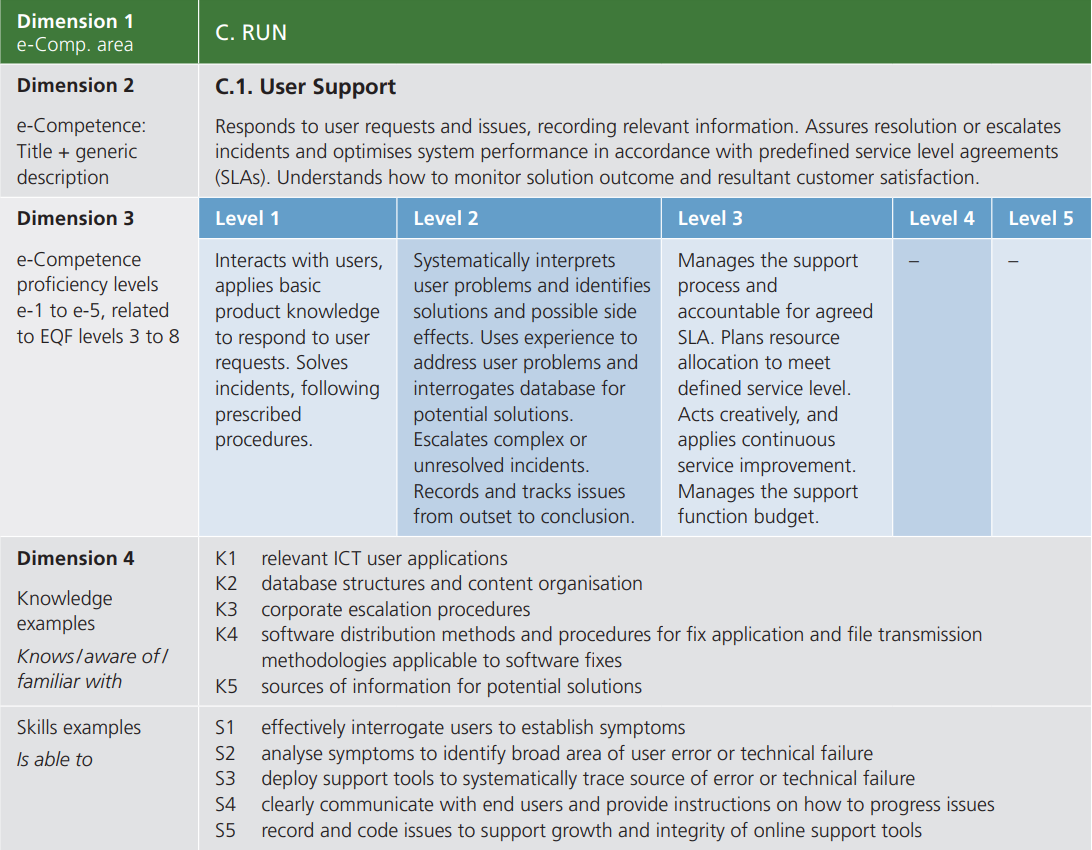
\includegraphics[width=0.9\textwidth]{user_support_ecf.png}
            \caption[short]{e-CF User Support role description}
            \label{fig:usersupportecf}
      \end{figure}
\end{center}


Figure \ref{fig:usersupportecf} illustrates the e-CF description of a technical role, presenting information in a clear and standardized manner. The left side of the figure is divided into several sections, as previously discussed. The first two sections provide a brief description of the role, emphasizing its connection to a specific business phase; in this specific figure, it is the operational phase known as RUN, indicative of day-to-day operations. Following that, the proficiency levels associated with the role are detailed. These levels can be roughly compared to the AEM Fiber levels, offering a standardized way to understand skill proficiency. The last element of the figure is a list of examples highlighting the essential knowledge and skills expected from an individual in the user support operator role.\\

Based on the indications of the domain expert, we determined that each AEM Fiber employee has to know how to deal with these issues, as presented in Figure \ref{fig:aemfibertasks}, according to their proficiency level: Configuration hosting mail, Connectivity disservice, POTS disservice, Input/output hosting mail, Connectivity degradation, SPAM, POTS degradation, VOIP disservice, VOIP degradation. The tasks in Figure \ref{fig:aemfibertasks} are in descending order of difficulty and the ability to solve them differs according to their difficulty level.

\begin{center}
      \begin{figure}[ht]
            \centering
            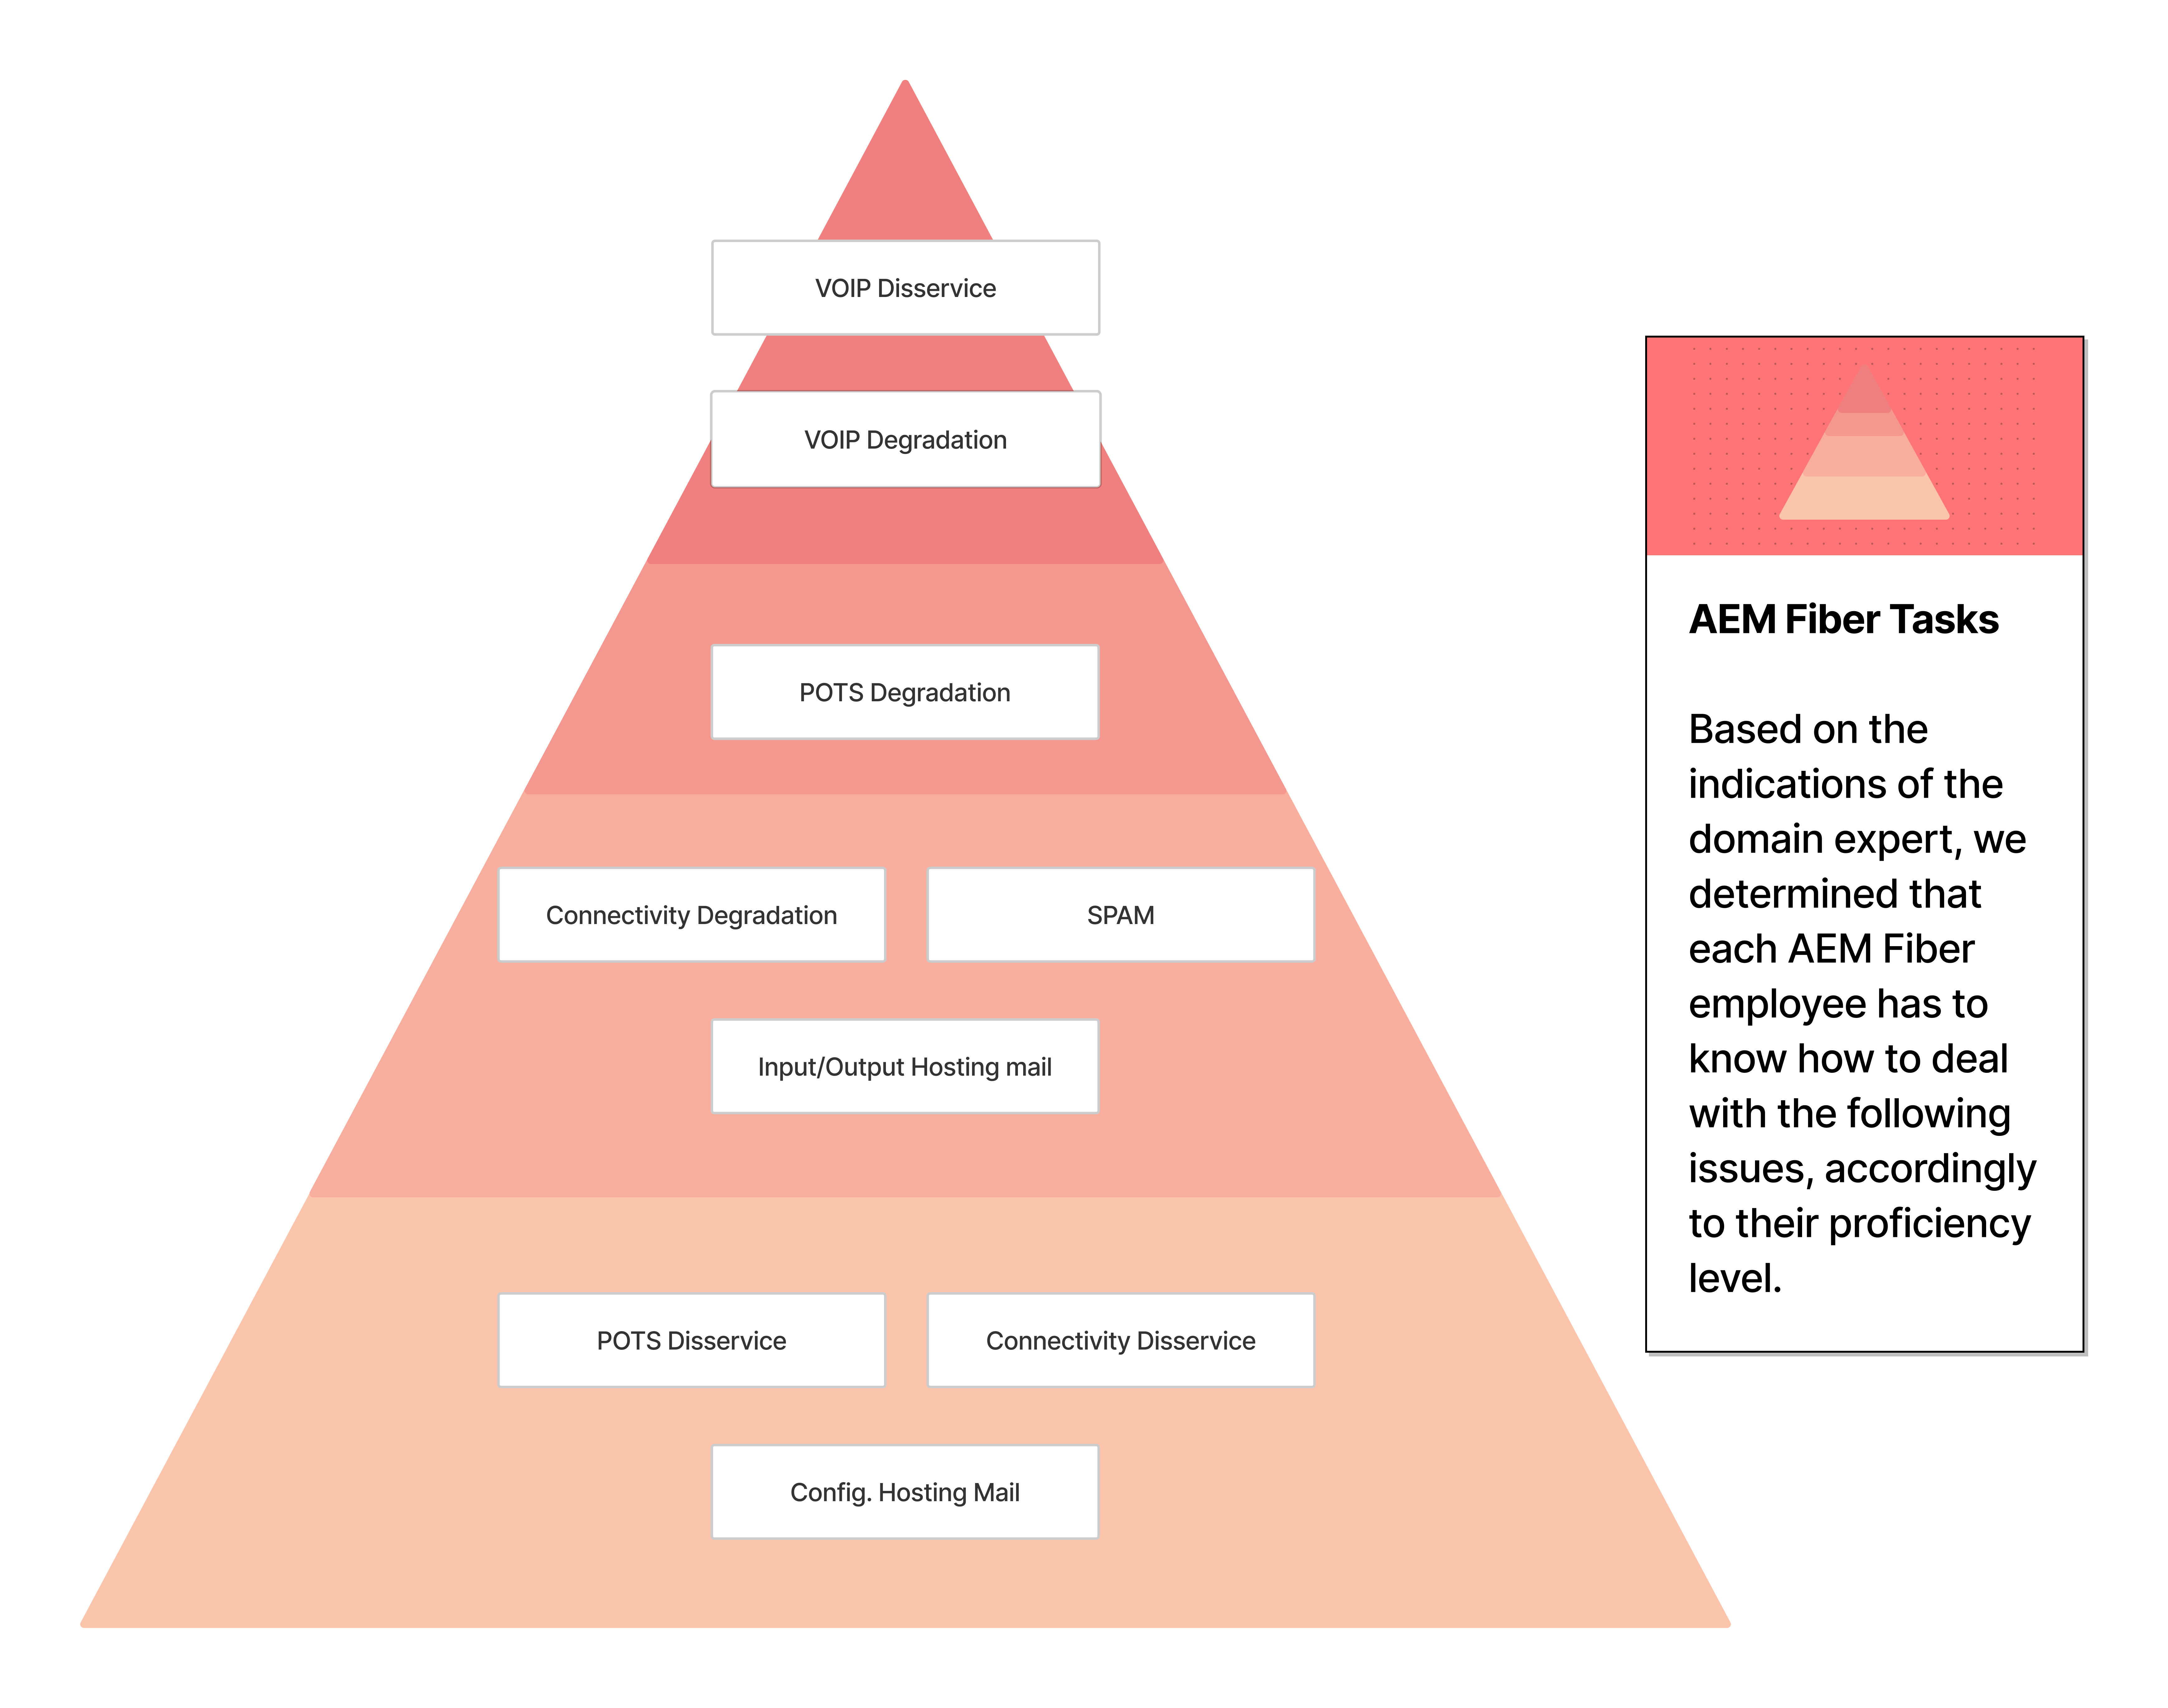
\includegraphics[width=0.9\textwidth]{aemfiber_tasks.png}
            \caption[short]{AEM Fiber task complexity pyramid}
            \label{fig:aemfibertasks}
      \end{figure}
\end{center}
\newpage

\section{Current AEM Fiber customer support workflow}

In Figure \ref{fig:aemfiberworkfloworiginal} we present the current AEM Fiber user support workflow process. In chapter \ref{sec:discussion} we will modify this workflow by adding the competence mapping phase, based on the results obtained during the experimental evaluation.

\subsection*{Call creation phase}

\begin{enumerate}
      \item Customer C calls the company support service to require assistance through the available communication channels.
      \item C is informed that the call will be recorded.
      \item The inbound call is assigned to Employee E.
      \item The dialogue between C and E is recorded.
      \item The call ends.
\end{enumerate}

\subsection*{Call update phase}

\begin{enumerate}
      \item Either Customer C or Employee E calls to provide/require updates on the reported issue.
      \item C is informed that the call will be recorded.
      \item The dialogue between C and E is recorded.
      \item The call ends.
\end{enumerate}

\begin{center}
      \begin{figure}[ht]
            \centering
            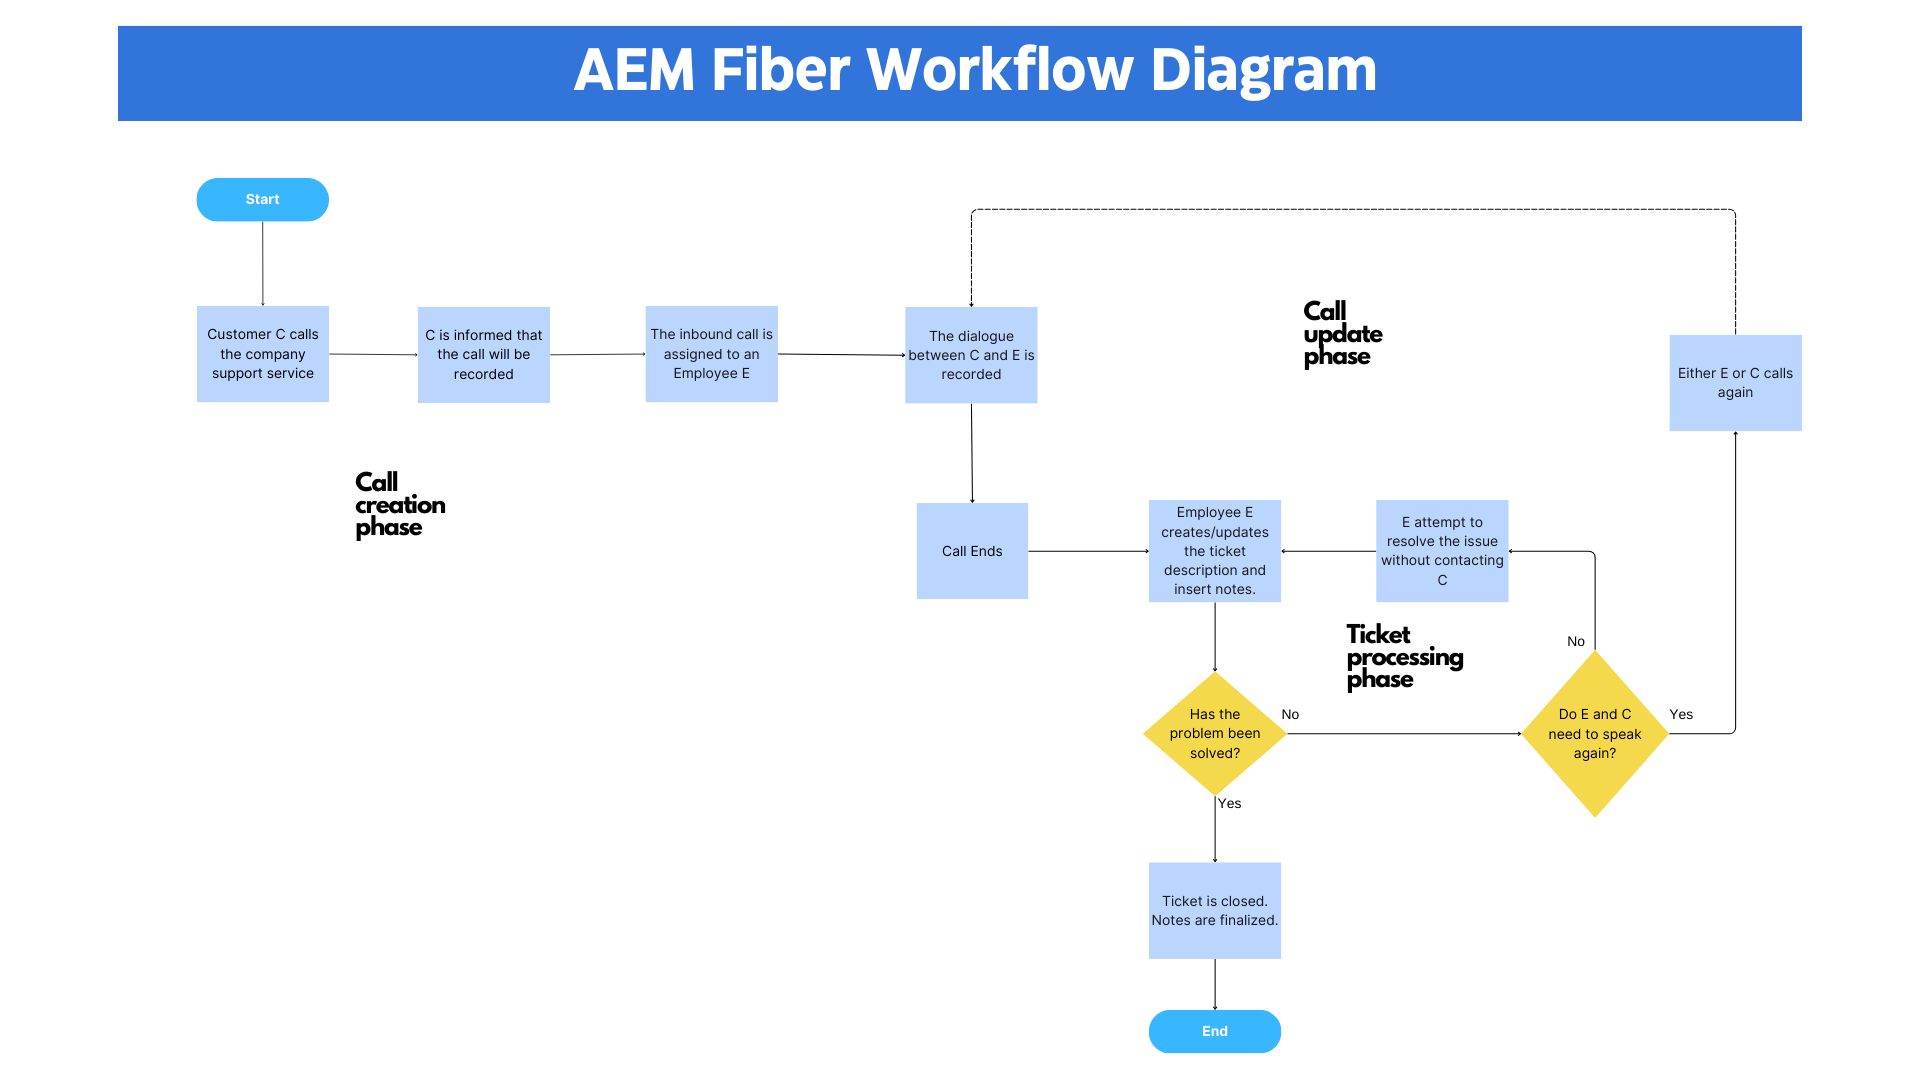
\includegraphics[width=1\textwidth]{workflow_original.png}
            \caption[short]{AEM Fiber customer support workflow}
            \label{fig:aemfiberworkfloworiginal}
      \end{figure}
\end{center}

\subsection*{Ticket processing phase}

\begin{enumerate}
      \item At the end of the first call (Call creation phase), employee E creates the ticket description.
      \item If needed the ticket is escalated from level 1 to level 2.
      \item After each operator's attempt to solve the issue or after any update call to/from the customer (Call update phase), new working notes are added to the existing ticket.
      \item When the problem has been solved and the customer is satisfied, notes are finalized and the ticket is closed.
\end{enumerate}

\section{Competence mapping in AEM Fiber}

Currently, AEM Fiber promotion system lacks a formal structure. Employees move up the levels based on management's assessment of their proficiency in resolving client issues and their ability to articulate themselves effectively. Typically, this advancement occurs after gaining experience within the company and by working on similar tasks daily. The decision on promotions heavily relies on the subjective judgment of the department manager, coupled with statistical data: the duration of customer calls, the number of resolved tickets, and the ticket categories are some of the metrics considered. However, these metrics only provide a partial view of employee competences and do not capture many aspects of their work. As a result, the manager's perspective plays a crucial role in the decision-making process. Additionally, the time an employee has spent at the company has a significant impact on promotion considerations.\\

As described in section \ref{sec:proposedframework}, our framework would extend the knowledge of the company on employee abilities, effectively improving the promotion system by incorporating a more comprehensive set of factors. Specifically, to evaluate the efficiency of a Large Language Model in the context of competence mapping we have decided to focus on a set of User Support macro-competences. Initially, we assess communication skills. This involves a detailed analysis of call transcripts handled by operators, utilizing the model to understand conversational dynamics. The objective is to evaluate the operators' proficiency in maintaining a friendly and clear communication style during calls. Subsequently, we delve into the evaluation of technical competences. This entails analyzing the user's request description to categorize it into specific subcategories based on ticket content. For instance, a "Hosting" ticket might be classified into subcategories like "Configuration Hosting Email" or "SPAM." By quantifying the successful resolution of tickets in each subcategory, we can comprehend the individual operators' skills. Each subcategory is also associated with a predefined difficulty level, as previously mentioned. Lastly, our framework includes an evaluation of problem-management competences. This involves analyzing the working notes generated by operators during the ticket resolution process to assess their ability to efficiently solve problems. While these three competences form the initial focus of our evaluation, it is important to acknowledge that additional competences may be identified. Given the academic nature of this paper, we are empirically testing and validating these competences within our proposed framework.

\section{Experimental evaluation}

We decided to use a transformer model for our tasks since it is the state-of-the-art architecture for NLP.
Due to the task at hand, we needed a generative model and decided to use GPT (Generative Pre-trained Transformer) thanks to its effectiveness at Closed Book Question Answering and Common Sense Reasoning.
In particular, we have chosen GPT3.5 because it was easily accessible, pre-trained on a vast set of examples, and ready to use. Since we couldn't access AEM Fiber data, we had to use external datasets for our experiments. We used \href{https://zenodo.org/records/4274454}{I-BiDaaS TID Synthetic Call Centre Dataset} to evaluate the communication competence and \href{https://data.milwaukee.gov/dataset/callcenterdatahistorical/resource/abdfe983-e856-40cd-bee2-85e78454344a}{Milwaukee City Call Center Dataset} for the technical competence evaluation. Together with the domain expert, we generated the working notes used to evaluate the problem management competence.

\subsection{Dataset description}
The first dataset is a simulated dataset comprising several simulated customer interactions with an agent representative, with both roles performed by actors. The scripting, both from customer and agent, aims to develop typical scenarios by Telco-oriented call center operations. Each record contains a transcription obtained by an automatic speech recognition system; the use of an automatic speech recognition system leads to dealing with some errors in the text (eg. incorrect transcription, missed speech parts)

\begin{quote}
      \label{transcription-nine}
      Tech: Movistar, good afternoon. This is Toledo speaking. Please tell me how I can assist you.

      Customer: Hello, good afternoon. I wanted to inquire about my current plan. I have one gigabyte of internet, and I want to know when I'll have the regular speed again after the usage is reset.

      Tech: Sure, in terms of billing cycles, your plan's usage resets from the 18th to the 17th of each month. I can check for you. The next reset will occur on the 18th of December, and you actually have two gigabytes included in your plan.

      Customer: I see. And if there hasn't been any usage yet?

      Tech: Let me check. Could you please provide me with the phone number for the other query?

      Customer: It's three four one nine eight zero five zero four nine eight.

      Tech: Alright. Let me check that line. Yes, that line ending in eighteen hasn't used any data yet.

      Customer: Yes, that's right. It's for my father, he has a non-internet phone. Is there any way to connect my line to his?

      Tech: I see. Well, if both lines have the same account holder, we can activate a shared data service at no additional cost. This way, you can share the data between the two lines.

      Customer: That's perfect. That's perfect.

      Tech: Alright, then. I'll activate it for you in just a moment, if you don't mind waiting.

      Customer: Okay.

      Tech: It's done for you now. In about five minutes, you'll be able to call and activate the service. So, both lines will have a total of four gigabytes to share.

      Customer: That's great. Thank you very much.

      Tech: You're welcome. Do you have any other questions or anything else we can help you with?

      Customer: No, just that.

      Tech: Alright, then. Thank you very much for the call. It was a pleasure assisting you.

      Customer: Very kind of you.

      Tech: Just a moment. They will call you to gather feedback on the service. Whenever you're available, feel free to provide your feedback. Have a good day.

      Customer: Thank you, you too.

      Tech: Thank you.
\end{quote}

In this scenario, the operator demonstrated kindness and effective communication skills in explaining information to the customer. Throughout the entire conversation, the operator maintained a professional and friendly approach. They were articulate in their explanations and successfully persuaded the customer to activate an additional service. From the perspective of customer satisfaction, it's evident that the customer was content by the conclusion of the conversation. This follows the guidelines of the company as explained by the domain expert. To better evaluate the model's ability to identify negative behaviors, we added some records to the dataset. These records featured actors simulating uncooperative customer-operator interactions, which required the model to recognize and respond to negative behaviors. An example of negative behavior is the following:

\begin{quote}
      Customer: Okay, okay. But is it for the same thing, or are they removing some service?

      Tech: No, we're not removing or adding any services. God how many time do I have to say this. It's for the same thing you have.

      Customer: Okay, okay no need to get agitated.

      Tech: Deal with it. Do you have any other questions?

      Customer: No, no.
\end{quote}

In this case, the operator is unclear and becomes unfriendly when the customer asks to clarify, which in turn makes the customer visibly uncomfortable. Such behavior clearly violates AEM Fiber guidelines and must be avoided or reported.

The second dataset contains information from the Milwaukee Call Center. It has six columns:
\begin{itemize}
      \item CREATION\_DATE: This shows when each request or call was made.
      \item OBJECT\_DESC: This column includes the location of the call, with the street address in Milwaukee, Wisconsin.
      \item TITLE: It categorizes each call into different categories, such as "Garbage Cart: Damaged."
      \item CLOSED\_DATETIME: This column records when the reported issue was resolved or closed, if applicable.
      \item CASE\_CLOSURE\_REASON\_DESCRIPTION: It explains why each case was closed, providing context for the resolution.
\end{itemize}
The dataset covers various issues, including garbage collection problems, street maintenance, and sanitation concerns. It is a record of interactions and issues reported to the Milwaukee Call Center, mirroring the issue report in our analyzed company.
\begin{center}
      \renewcommand{\arraystretch}{1.5}
      \begin{tabularx}{\textwidth}{l|X}
            \toprule
            TITLE           & CASE\_CLOSURE\_REASON\_DESCRIPTION                                                                                                                                                                                                                                                                                                                               \\
            \midrule
            All Other Signs & On Kearney St, there is a “No Left Turn” sign that was put up during the state fair, which I believe was intended to be temporary. The attached image shows where the sign is, although the “No left turn” sign is not present in the picture.                                                                                                                   \\
            \hline
            Pothole         & Heading southbound, in the right turn lane.                                                                                                                                                                                                                                                                                                                      \\
            \hline
            Pothole         & There was a chunk of pavement that popped out, looked like the resulting hole was beside a manhole in the southbound lane (76th). I believe the location of the pothole is within 20 ft of Stevenson St intersection. The chunk of pavement was no longer in traffic later in the day when I drove past again later in the day, so that aspect is not a concern. \\
            \hline
            Area Dark       & No light for a few months ago.                                                                                                                                                                                                                                                                                                                                   \\
            \hline
            One Way Sign    & Northbound on 76th, at O'Connor. One Way sign top bolt missing and sign is falling down. Attached picture shows the sign needing attention, although it is not falling down in the picture as it is an older picture from Google maps.                                                                                                                           \\
            \bottomrule
      \end{tabularx}
\end{center}

In AEM Fiber, the operators initiate their task by creating a summary equivalent to the OBJECT\_DESC value. After interacting with the customer, each operator is required to articulate the problem in a ticket description and select the relevant category. Accurate classification of each ticket holds significant importance for AEM Fiber, as it provides a clear insight into the company issues. Furthermore, a more detailed classification, including subcategories within each main category, would enhance the ability to evaluate each employee's performance based on their successfully resolved tickets.
For the third competence we tried searching for datasets that could contain transcriptions of work notes, but we couldn't find any that met our requirements. That's why we decided to generate our own work notes, thanks to the suggestions given by the domain expert about their structure and their general content. In particular, we wrote these notes directly in Italian language since AEM Fiber is an Italian company: in the real case, in fact, the operators write the notes in Italian.
Each work note contains the date, name of the technician who wrote the note, and the relative content; in particular, the latter contains all the steps of the problem management process. The domain expert told us that usually, the operators don't follow a proper structure while writing these notes. \label{sec:datasetProblemManagement}
Here we present some work note examples (translated into English).
\begin{itemize}

      \item First example

            14/09/23 08:00\\
            Operator 1\\
            Taken in charge, starting to check\\

            14/09/23 08:30\\
            Operator 1\\
            The line is working correctly, but the router is malfunctioning. Proceeding with replacement of it.\\

            15/09/23 11:30\\
            Operator 1\\
            Customer has received the router and confirms proper functionality.
\end{itemize}
In this case, the operator \textit{correctly} understands that the client's problem is about the router; that's why he decides to replace it. This perfectly fits with the company's guidelines and, since he also understood immediately the problem, this is an example of good problem management.
\begin{itemize}
      \item Second example

            14/08/2023 15:00\\
            Operator 4\\
            I take charge of the ticket.\\

            14/08/2023 15:15\\
            Operator 4\\
            The customer reports having slow connection only with wifi devices, but upon checking with tools, it seems there is an issue at the central office level. I involve the external technician so they can inspect the external central office.\\

            15/08/2023 16:00\\
            Operator 4\\
            Following the inspection of the external central office, the external technician informs me that there is no problem detected up to the main telephone socket, indicating that the issue is related to the internal installation. I contact the customer and agree on the replacement of the router.\\

            17/08/2023 10:30\\
            Operator 4\\
            The customer has received the router and connected it. They attempt a browsing test and report that it is working correctly. I ask them to monitor it and contact us in case of any issues. The closure of the report is agreed upon.
\end{itemize}

In this case, the operator \textit{wrongly} interprets the problem as an external one; this leads to the technician being sent to the central office unnecessarily. This is a serious issue for AEM Fiber because it means losing time and paying the external technician without him solving a real problem. So this is a bad example of problem management.
\chapter{Results}
\label{sec:results}

We will now proceed to discuss our experimental results. As described more in detail in the technical appendix \ref{sec:techappendix}, GPT offers valuable capabilities but it does come with certain limitations. Its proficiency in analyzing communication is fine, although it may not consistently detect specific behavioral patterns within the transcription; additionally, the model tends to exhibit a bias towards recognizing positive behaviors (kindness, professionality, etc.) in conversations, often assigning high scores even when an operator's responses are deemed unacceptable accordingly to the company guidelines. In our experiments we considered only a subset of communication-related indicators, however, it is our belief that other indicators in this context may yield similar results: despite the advancements in Natural Language Processing (NLP), the capacity of Large Language Models to thoroughly analyze human conversation remains relatively limited. While models like GPT exhibit an ability to comprehend the overall meaning, their precision lowers when tasked to evaluate the conversation according to specific indicators. In addition, the company needs to rely on an automated transcription process to obtain the transcription data, which introduces noise and leads to worse performances. \\

GPT is much more reliable in assessing technical competences, where it exhibits an excellent ability to identify pertinent information, such as the location of an issue in the provided ticket description, as observed while testing GPT on the Milwaukee dataset. Moreover, it showcases a strong capability of precisely categorizing different types of tickets. \\

In problem-solving scenarios, GPT performs well, as its primary objective is to understand whether prescribed processes (e.g. the company's guidelines) have been followed, rather than understanding complex language dynamics. Thus, in such scenarios, GPT proves to be a valuable asset; however, it is important to acknowledge that its performance may vary depending on the specific task at hand and the nature of the data being processed.

\section{Communication competence}

To explore more in-depth the possible impact of Competence Mapping on AEM Fiber we will proceed with the \textcolor{orange}{GPT} analysis of the examples illustrated in the previous sections, starting with the communication competence.\\

\textbf{GPT's analysis of the positive behavior transcription}: In this customer service interaction with Movistar, the tech representative, Toledo, comes across as courteous and professional. Toledo starts the conversation with a friendly greeting and maintains a positive tone throughout. The clarity of explanation is notable as Toledo provides precise details about the customer's plan, billing cycle, and upcoming data reset date. The customer seems satisfied, expressing appreciation with phrases like "That's perfect." This suggests that the customer's needs were effectively addressed. What stands out is the tech representative's ability to identify an opportunity for upselling. Toledo suggests activating a shared data service for the customer's father's non-internet phone, adding value to their plan at no extra cost. The customer responds positively, indicating successful upselling. The overall flow of the conversation is smooth, and Toledo manages to not only solve the customer's initial query but also enhance their plan, contributing to a positive customer experience. The interaction concludes on a polite note, with Toledo thanking the customer and encouraging them to provide feedback when contacted later, reinforcing a customer-centric approach.\\

\textbf{GPT's analysis of the negative behavior transcription}: In this interaction, the tech representative, Asunta, initially greets the customer politely but the conversation takes a tense turn when discussing a price change. The customer mentions a shift from sixty to seventy-five euros, but Asunta insists it's only a five-euro increase, leading to some confusion and frustration. The conversation becomes more strained as the customer questions the amount and the tech representative responds assertively. Asunta requests the customer's landline number to verify the details and eventually confirms the correct tariff, emphasizing that the increase is indeed just five euros. There's a notable lack of patience and empathy in Asunta's responses, with phrases like "Why are you even arguing with me?" and "Deal with it." Despite this, the customer seems to accept the clarification toward the end of the conversation. The interaction doesn't involve upselling or promoting additional services. Instead, it focuses on resolving the customer's concern about the price increase. Overall, while the issue is addressed, the tone may impact customer satisfaction negatively, and the tech representative's approach could be improved for a more positive customer experience.\\

The insights provided by the model are particularly valuable for the company's customer service strategy. In the positive transcription, the model accurately identifies that a friendly tone is maintained while resolving the issue, emphasizing the importance of ensuring customer comfort throughout the interaction. Explanation clarity is rightly acknowledged as a crucial factor, directly influencing the efficiency of both the operator and the company as a whole. Clear communication contributes to a positive customer experience and reflects well on the company's professionalism. The model also draws attention to the operator's ability to make a pitch sale, showcasing their initiative. This is pivotal as it not only resolves the customer's issue but also presents an opportunity to enhance the customer's experience, showcasing proactive service. In the negative case, the model aptly notes that even after resolving the issue, if the customer doesn't feel comfortable, it may lead to reluctance to seek the company's services again. Additionally, the model identifies a lack of empathy in the negative scenario, emphasizing the importance of adapting explanations when the customer is struggling to understand. This insight highlights the significance of empathy in customer service, ensuring a positive and supportive interaction even in challenging situations. In summary, the model's analysis not only captures the technical aspects of issue resolution but also delves into the non-technical aspects as requested. These insights will contribute to refining and enhancing the company's customer support practices.

\section{Technical Competence}

In this case, the task was to extract information from the text without the need to understand complex language dynamics.
Overall both category and subcategory extraction were successful. Usually, the confusion stems from the similarity between subcategories, creating challenges for both humans and GPT in determining the correct category. It is also hypothesized that multiple correct categories may exist in some instances. To assess the model's ability to recognize the location mentioned in the ticket request, a comparison was made between GPT's response and manually extracted labels. In most cases, GPT accurately identified the correct street or set of streets, even though it occasionally struggled with inferring street types (e.g., Street, Avenue, Boulevard). Approximately 90\% of the time, the correctness of the produced string exceeded the acceptable score. Furthermore, the majority of cases resulted in a perfect score, indicating that the model is generally proficient in identifying the mentioned street.

\section{Problem Management competence}

We will now proceed with the analysis of the examples of Problem Management competence illustrated in the previous sections.\\

\textbf{GPT's analysis of Ticket 1}: Operator 1 demonstrated prompt and professional handling of the reported issue on 14/09/23 at 08:00. They efficiently diagnosed a malfunctioning router by 08:30 and promptly decided to replace it, showcasing technical expertise and a commitment to swift issue resolution. On 15/09/23 at 11:30, the customer confirmed receiving the replacement router and verified its proper functionality, reflecting effective communication and end-user satisfaction.

Throughout the incident resolution process, Operator 1 maintained professionalism. The issue was resolved within a day, from identification on 14/09/23 to confirmation on 15/09/23. Timely updates were provided to the customer, contributing to a well-informed and satisfied end user.

While the specific origin of the problem—whether internal or external—was not explicitly stated, the decision to replace the router suggested a focus on addressing potential internal system issues. The necessity to replace the router underscored a proactive approach to rectifying the malfunction and ensuring the long-term stability of the customer's network setup.

Importantly, there was no need to involve an external field technician, indicating Operator 1's self-sufficiency in managing and resolving the reported issue. This further emphasized their technical proficiency and the effectiveness of the troubleshooting and replacement processes.\\

\textbf{GPT's analysis of Ticket 2}: Operator 4 appeared to handle the situation professionally. The resolution of the issue took three days, which is equal to or greater than two days. Throughout the process, the customer was kept informed of the ticket's status. The problem was initially suspected to be at the central office level, leading to the involvement of an external technician. However, after inspecting the external central office, the technician found no issues, indicating that the problem was related to the internal installation. Consequently, the customer was contacted, and an agreement was reached to replace the router. Once the customer received and connected the new router, they conducted a browsing test, reporting that it worked correctly. The operator advised them to monitor the situation and reach out in case of any issues. It's noteworthy that the on-field technician was not required since the problem was traced back to the internal installation, specifically the router. As we commented for the communication competence, the insights provided by GPT are particularly interesting for the company's customer service strategy.\\

As we commented for the communication competence, the insights provided by GPT are particularly interesting for the company. GPT correctly identifies that the first operator has worked in a professional way, by understanding the problem and also keeping the client updated: this means that the operator can solve issues by carefully following the company's guidelines. In the second ticket GPT can clearly distinguish two different aspects: as underlined, the operator has required the on-field technician in vain, but at the same time he still remained professional in terms of how he handled the communication with the client. So, by pinpointing instances where operators effectively resolve issues while adhering to guidelines, the company can refine problem-solving procedures, optimize operational efficiency, and ensure consistent high-quality service, ultimately leading to improved customer satisfaction.\\

As detailed in the Technical Appendix \ref{sec:techappendix}, we introduced a system where each response generated by GPT is assigned a numerical weight based on its significance. For instance, a score of 1 might be given to an operator displaying professionalism, while a score of 3 could be assigned if the operator successfully resolves an issue within 48 hours. This approach allows us to quantify and prioritize the effectiveness of each operator. In particular, as we said before, a very important aspect to consider (for AEM Fiber) is to check whether the operator has unnecessarily called the external technician; to extract this information, we made a comparison between GPT understanding of the problem's nature (internal/external) and the action of the operator in this context. So, for example, if the problem was external and the operator called the technician, then this is good and we assign a high value, while if the problem was internal and the operator still called the technician, this means assigning a very low (negative, in our case) weight. Then these weights could be summed up to obtain a  result \texttt{ticketOperator\_$X_1 Y_1$} about that operator (identified as Y1) in relation to that ticket (identified as X1). Subsequently, there can be an aggregation method, like the sum, to obtain the final value for the operator Y1, in terms of problem management, based on all the tickets he has solved in a certain period of time: \texttt{finalValueOperator\_$Y_1$}.  For n tickets operator 1 has solved
\begin{equation}
      \texttt{finalValueOperator\_$Y_1$} = \sum_{i=1}^{n} \texttt{ticketOperator\_$X_i Y_1$}
\end{equation}
Also, a comparison of all the operators in terms of \texttt{finalValueOperator\_$Y_i$} can be done.\\

\section{Result's summary}
Our analysis of the results underscores the importance of exercising caution when contemplating the deployment of GPT within a competence mapping framework in a production environment, specifically when handling the communication competence. While our findings suggest areas where improvements may be needed, it's worth noting that GPT could offer significant value as an auxiliary tool, particularly in Human Resources (HR) applications.
\chapter{Discussion}
\label{sec:discussion}

In this chapter, we explore how competence mapping integrates into the AEM Fiber customer support workflow. We discuss the phases of call creation, update, and ticket processing, explaining how data related to %\textcolor{orange}{maybe is not a matter of "data from" but like \textit{related to }}
these stages help extract communication, technical, and problem-management competences. We also present a straightforward design for a competence mapping dashboard designed to assist HR and management in evaluating departmental and individual performance. This chapter expands on the ideas discussed in Chapter \ref{sec:results}.

\section{Competence mapping integration in case study customer support workflow}

The following is the updated AEM Fiber customer support workflow.

\begin{figure}[ht]
      \centering
      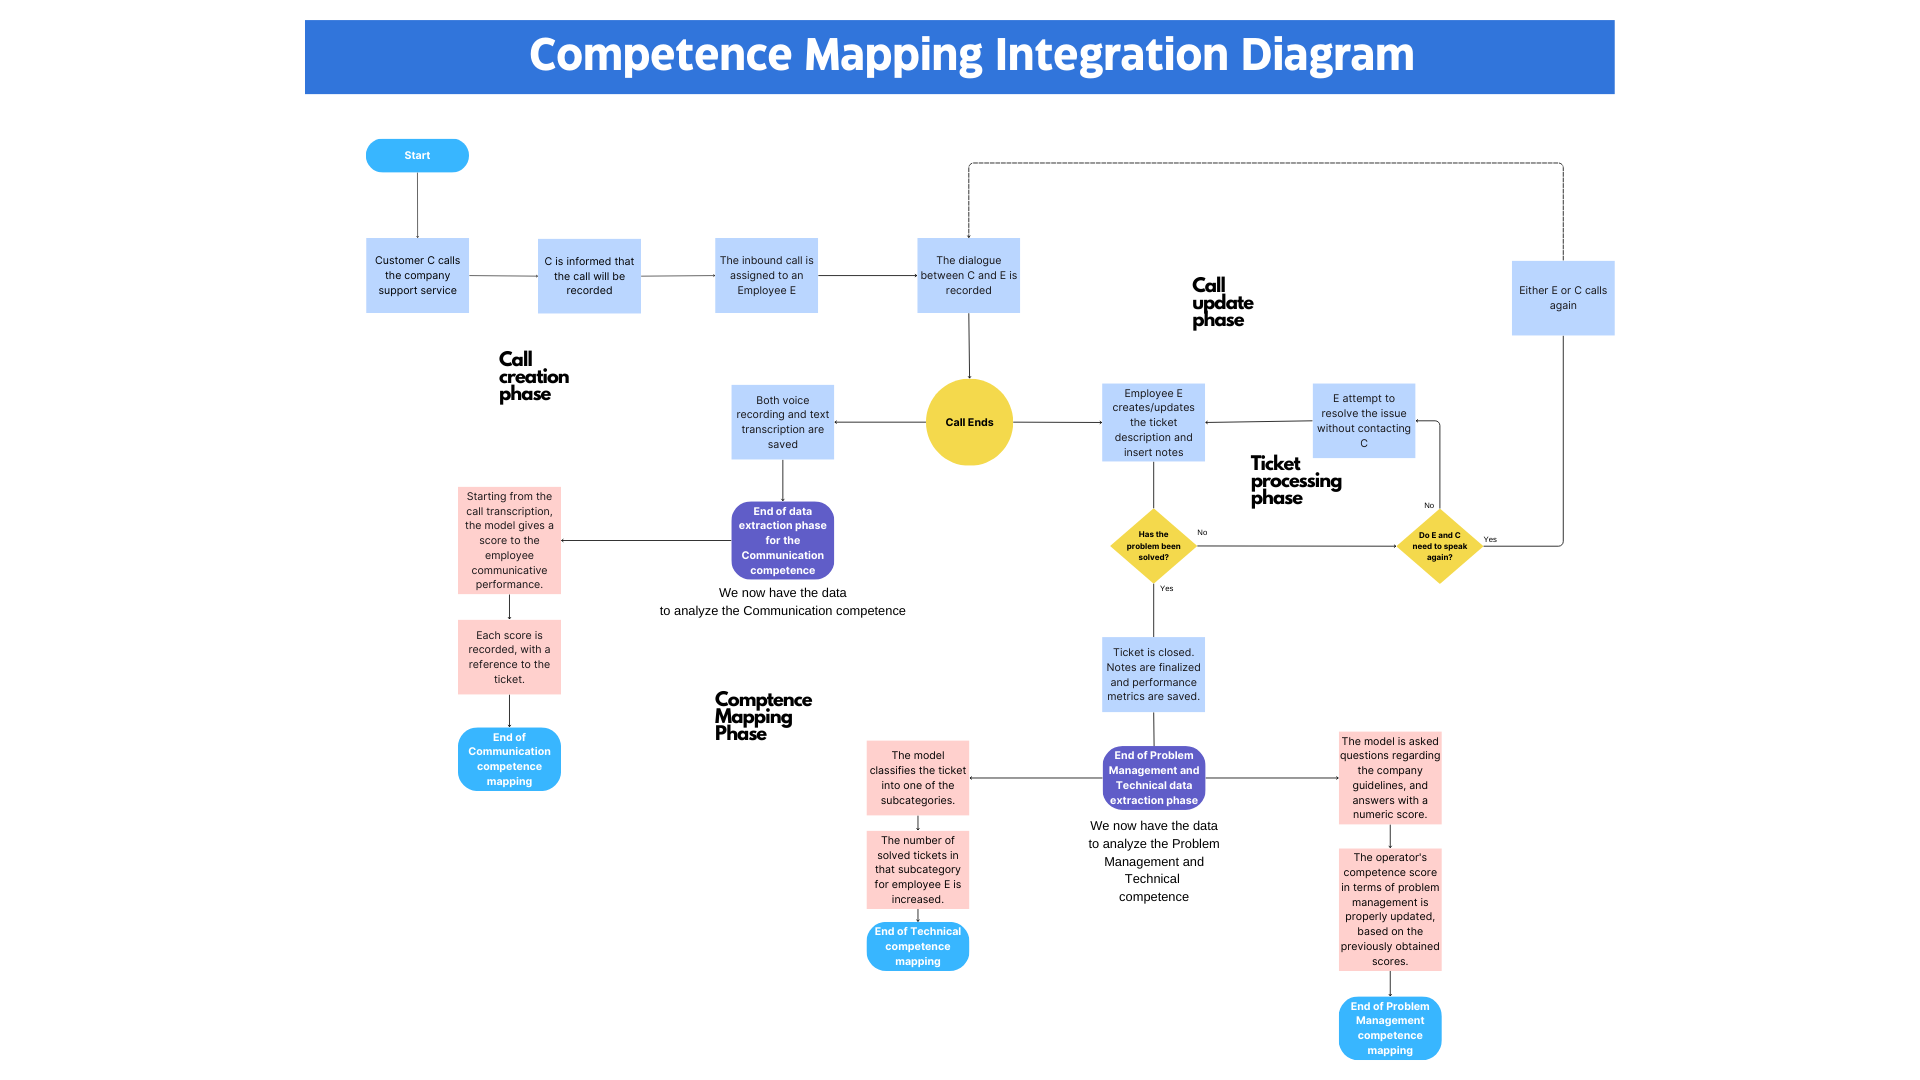
\includegraphics[width=\textwidth]{workflow_integrated.png}
      \caption{Competence mapping updated workflow}
      \label{figure:workflow_integrated}
\end{figure}

\subsection{Call creation phase}

\begin{enumerate}
      \item Customer C calls the company support service to require assistance through the available communication channels.
      \item C is informed that the call will be recorded.
      \item The inbound call is assigned to Employee E.
      \item The dialogue between C and E is recorded.
      \item The call ends.
      \item We have now all the data needed for the communication competence extraction.
\end{enumerate}

\subsection{Call update phase}

\begin{enumerate}
      \item Either Customer C or Employee E calls to provide/require updates on the reported issue.
      \item C is informed that the call will be recorded.
      \item The dialogue between C and E is recorded.
      \item The call ends.
      \item We have now all the data needed for the communication competence extraction.
\end{enumerate}

\subsection{Ticket processing phase}

\begin{enumerate}
      \item At the end of the first call (Call creation phase), employee E creates the ticket description.
      \item If needed the ticket is escalated from level 1 to level 2.
      \item After each operator attempts to solve the issue or after any update call to/from the customer (Call update phase), new working notes are added to the existing ticket.
      \item When the problem has been solved and the customer is satisfied, notes are finalized and the ticket is closed.
      \item At this point, we have all the data needed to extract the Technical and Problem Management competences.
\end{enumerate}

\subsection{Communication competence score extraction}

\begin{enumerate}
      \item Starting from the call transcription, the model gives a score to the employee's communicative performance.
      \item Each score is recorded, with a reference to the ticket.
\end{enumerate}

\subsection{Technical competence score extraction}

\begin{enumerate}
      \item As previously specified, the domain expert has provided a list of the possible subcategories for the ticket categorization, each associated with a difficulty level.
      \item The model classifies the ticket into one of the subcategories.
      \item The number of solved tickets in that subcategory for employee E is increased.
\end{enumerate}

The subcategory difficulty can be useful to understand how well an employee is learning.
We expect that Level 1 employees with longer tenures in the company will be less inclined to escalate simpler tasks to higher levels. The difficulty level can also be useful to compare the proficiency level in different tasks. If the task is considered difficult, a lower score can be considered a good score (e.g. 3.3/4 can be considered very good for a difficult task, but not enough for an easy one).

\subsection{Problem Management score extraction}

\begin{enumerate}
      \item As previously specified, the domain expert has provided a guideline regarding the key points that have to be followed during the problem resolution.
      \item The model is asked questions regarding the provided guideline; each answer corresponds to a certain score.
      \item The operator's competence score in terms of problem management is properly updated, based on the previously obtained scores.
\end{enumerate}

If the ticket has been escalated from level 1 to level 2, only the level 2 employee working notes are taken into consideration while producing the problem management score.

\section{Possible design of the competence mapping dashboard}

To better support HR and higher-level management, we've introduced a straightforward performance dashboard. Here, managers can access both general department metrics and specific details for individual employees. The left side of the dashboard displays competence evaluations for each employee. On the right, managers can compare employees using scatterplots based on various KPIs. This comparison aids in identifying high-performing employees for potential promotion and those needing additional training, as can be seen in Figure \ref{figure:recap}. Clicking on an employee's name reveals a detailed view, summarizing overall performance and listing the most recent assigned tickets. Managers can further analyze each competence by clicking the detail button, as shown in Figure \ref{figure:employee_overall}. Within the detailed competence view, sub-competences are broken down for a closer look. For instance, the communication competence is presented with graphs detailing specific strengths and areas for improvement. This straightforward approach equips managers with the necessary insights for departmental and individual performance assessments, as detailed in Figure \ref{figure:employee_detail}.

\vfill

\begin{figure}[ht]
      \centering
      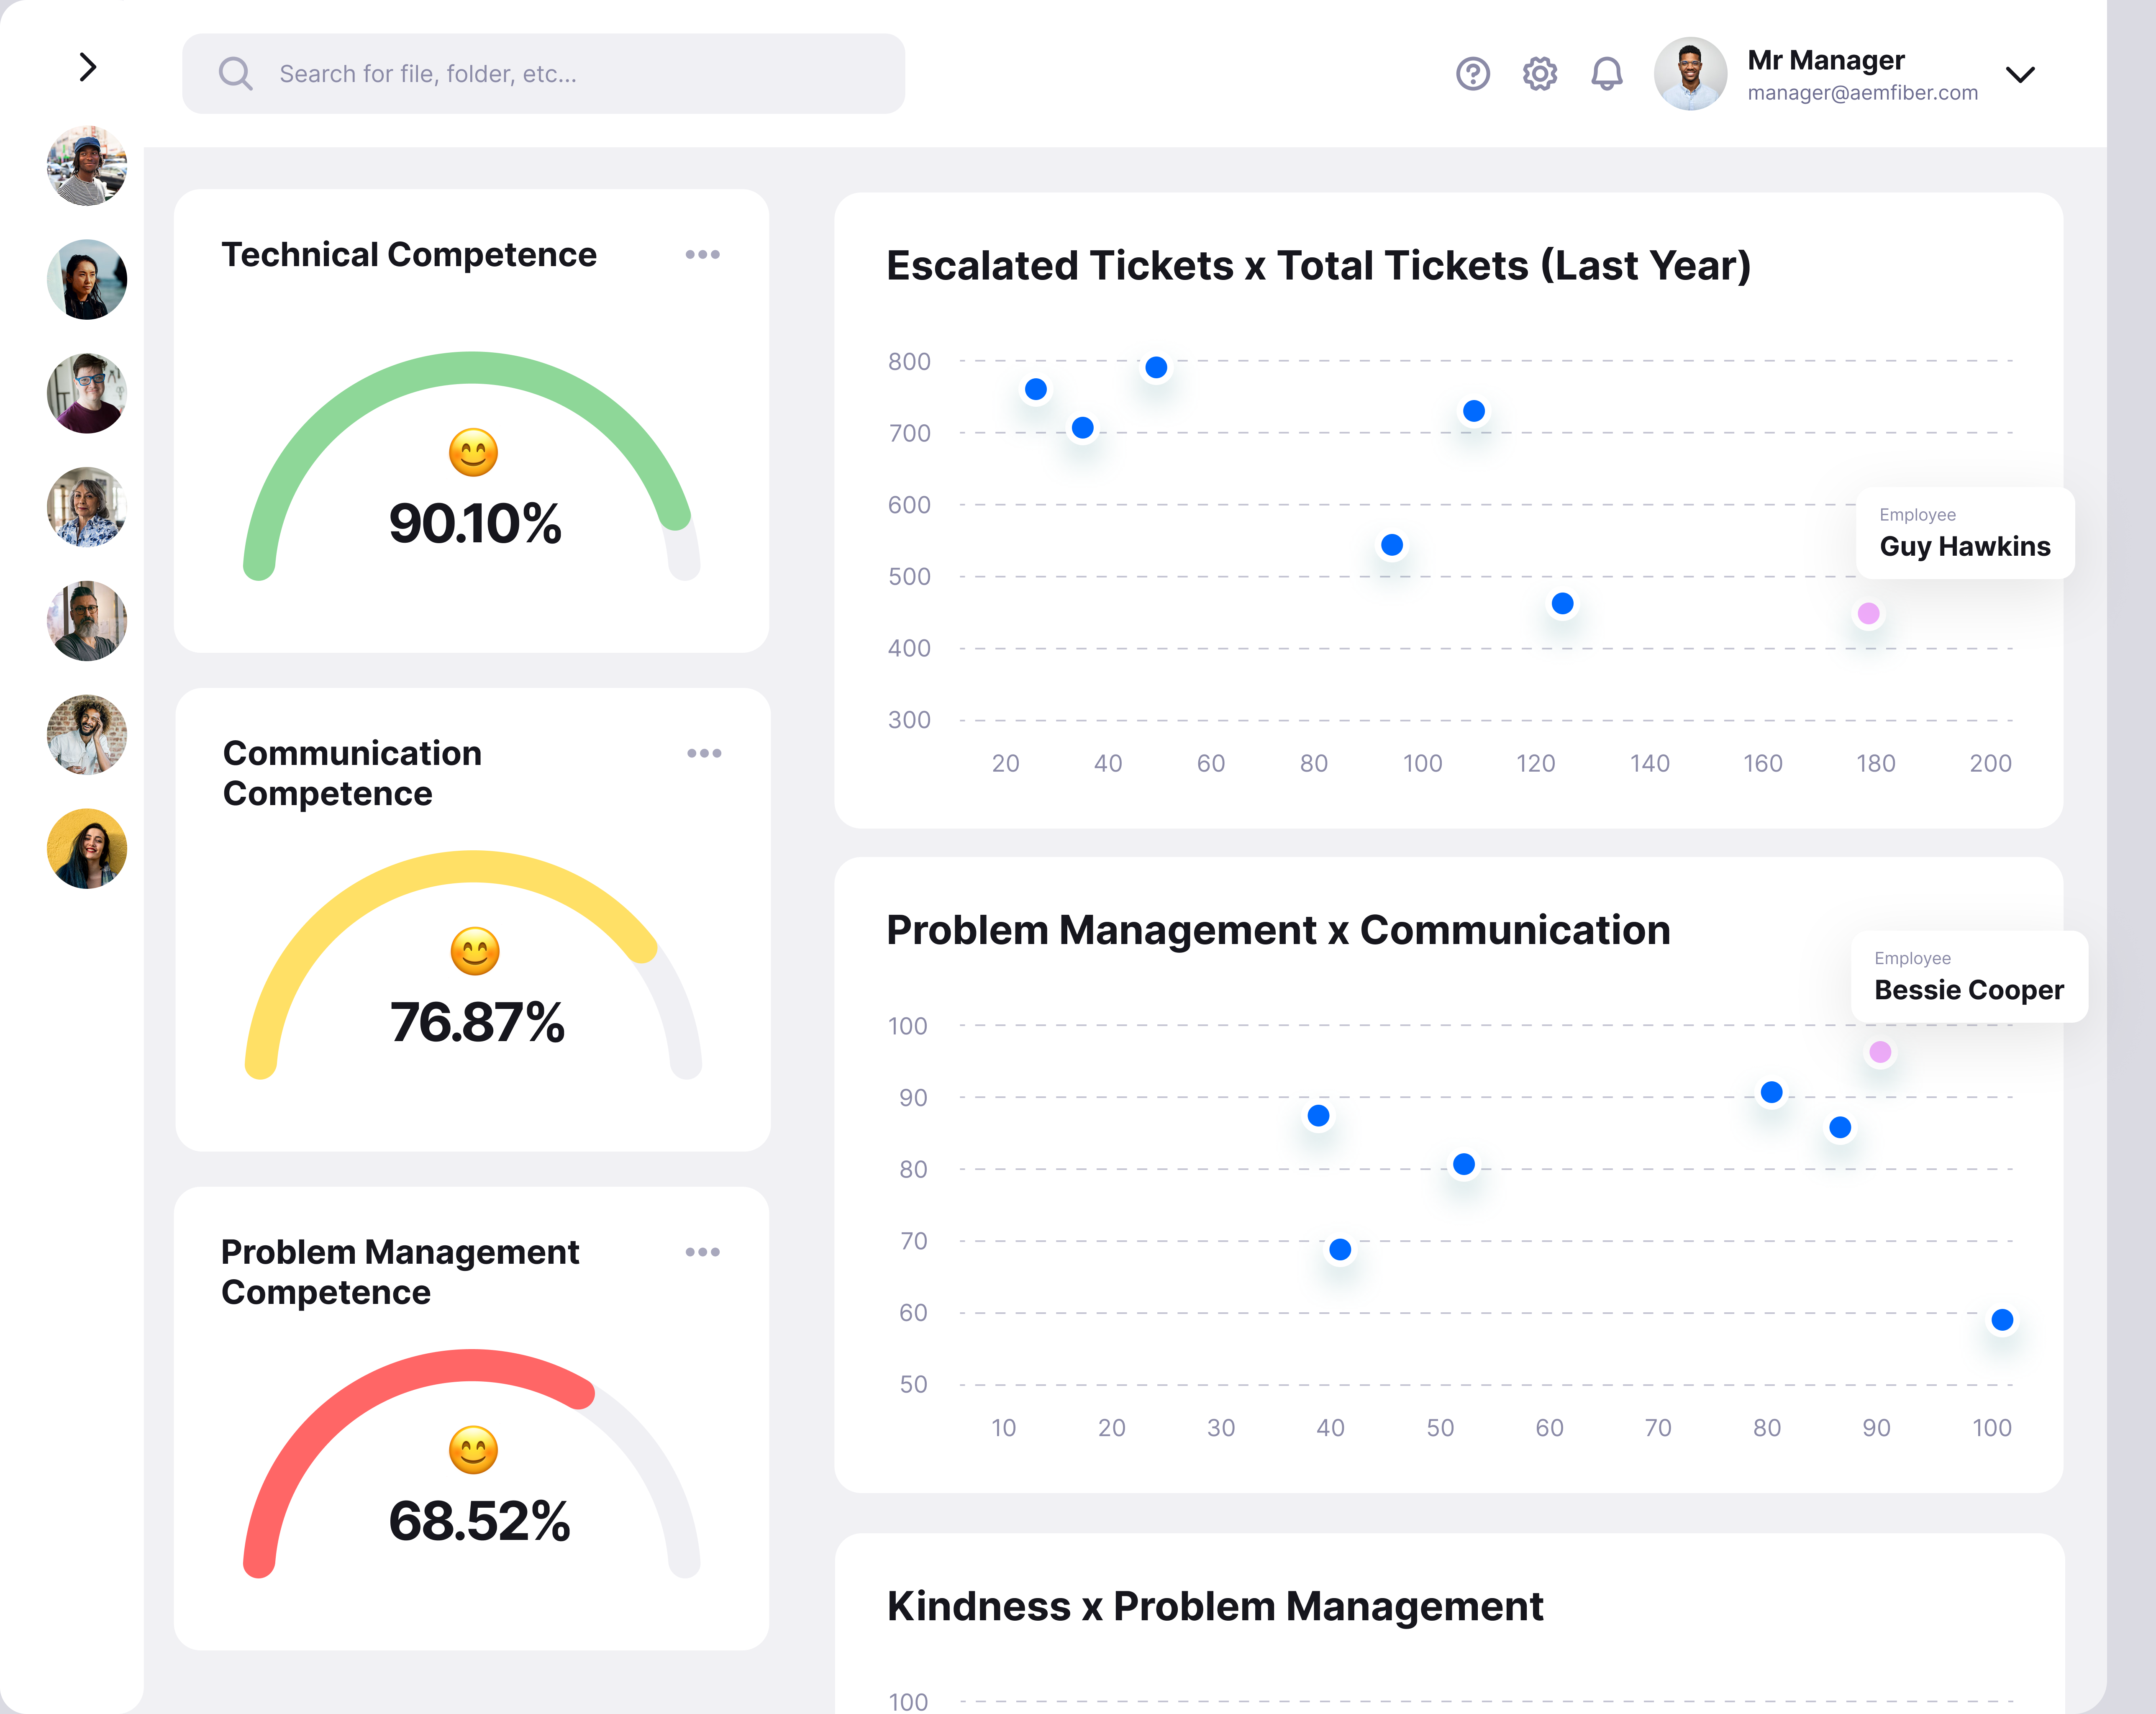
\includegraphics[width=\textwidth]{recap.png}
      \caption{Dashboard performance recap mock-up}
      \label{figure:recap}
\end{figure}

\vfill

\begin{figure}[ht]
      \centering
      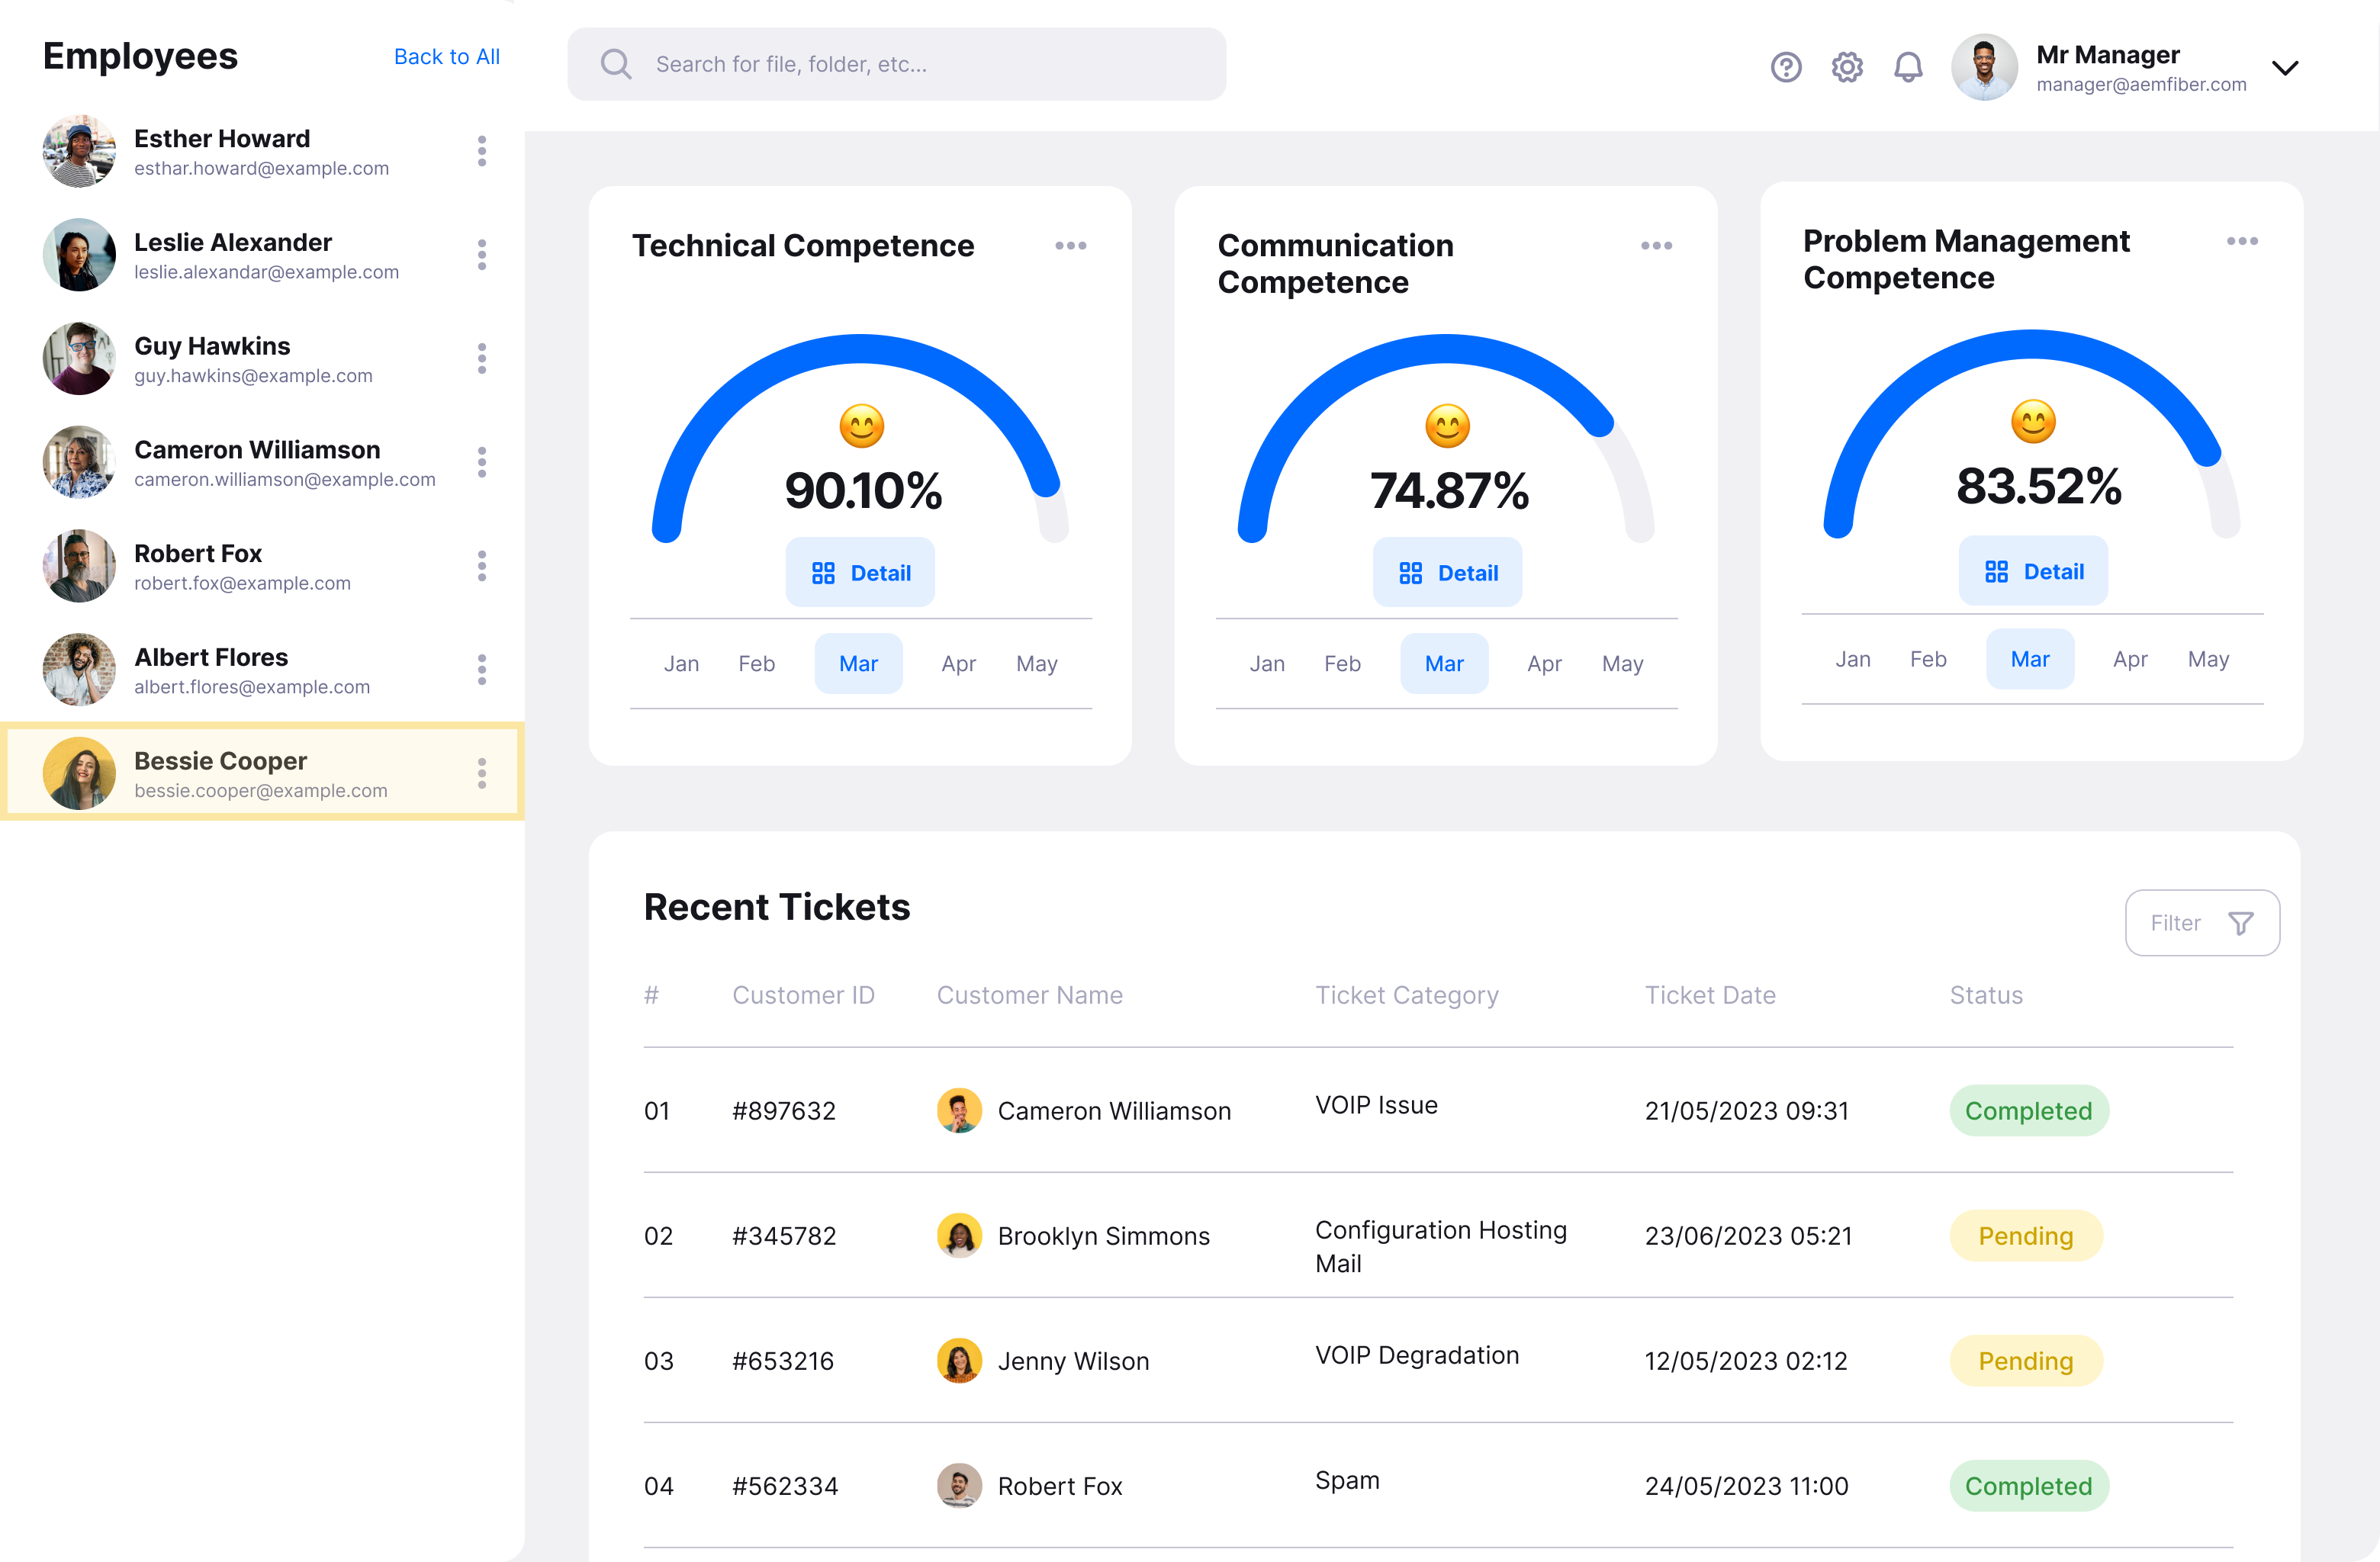
\includegraphics[width=\textwidth]{employee overall.png}
      \caption{Dashboard employee performances mock-up}
      \label{figure:employee_overall}
\end{figure}
\begin{figure}[ht]
      \centering
      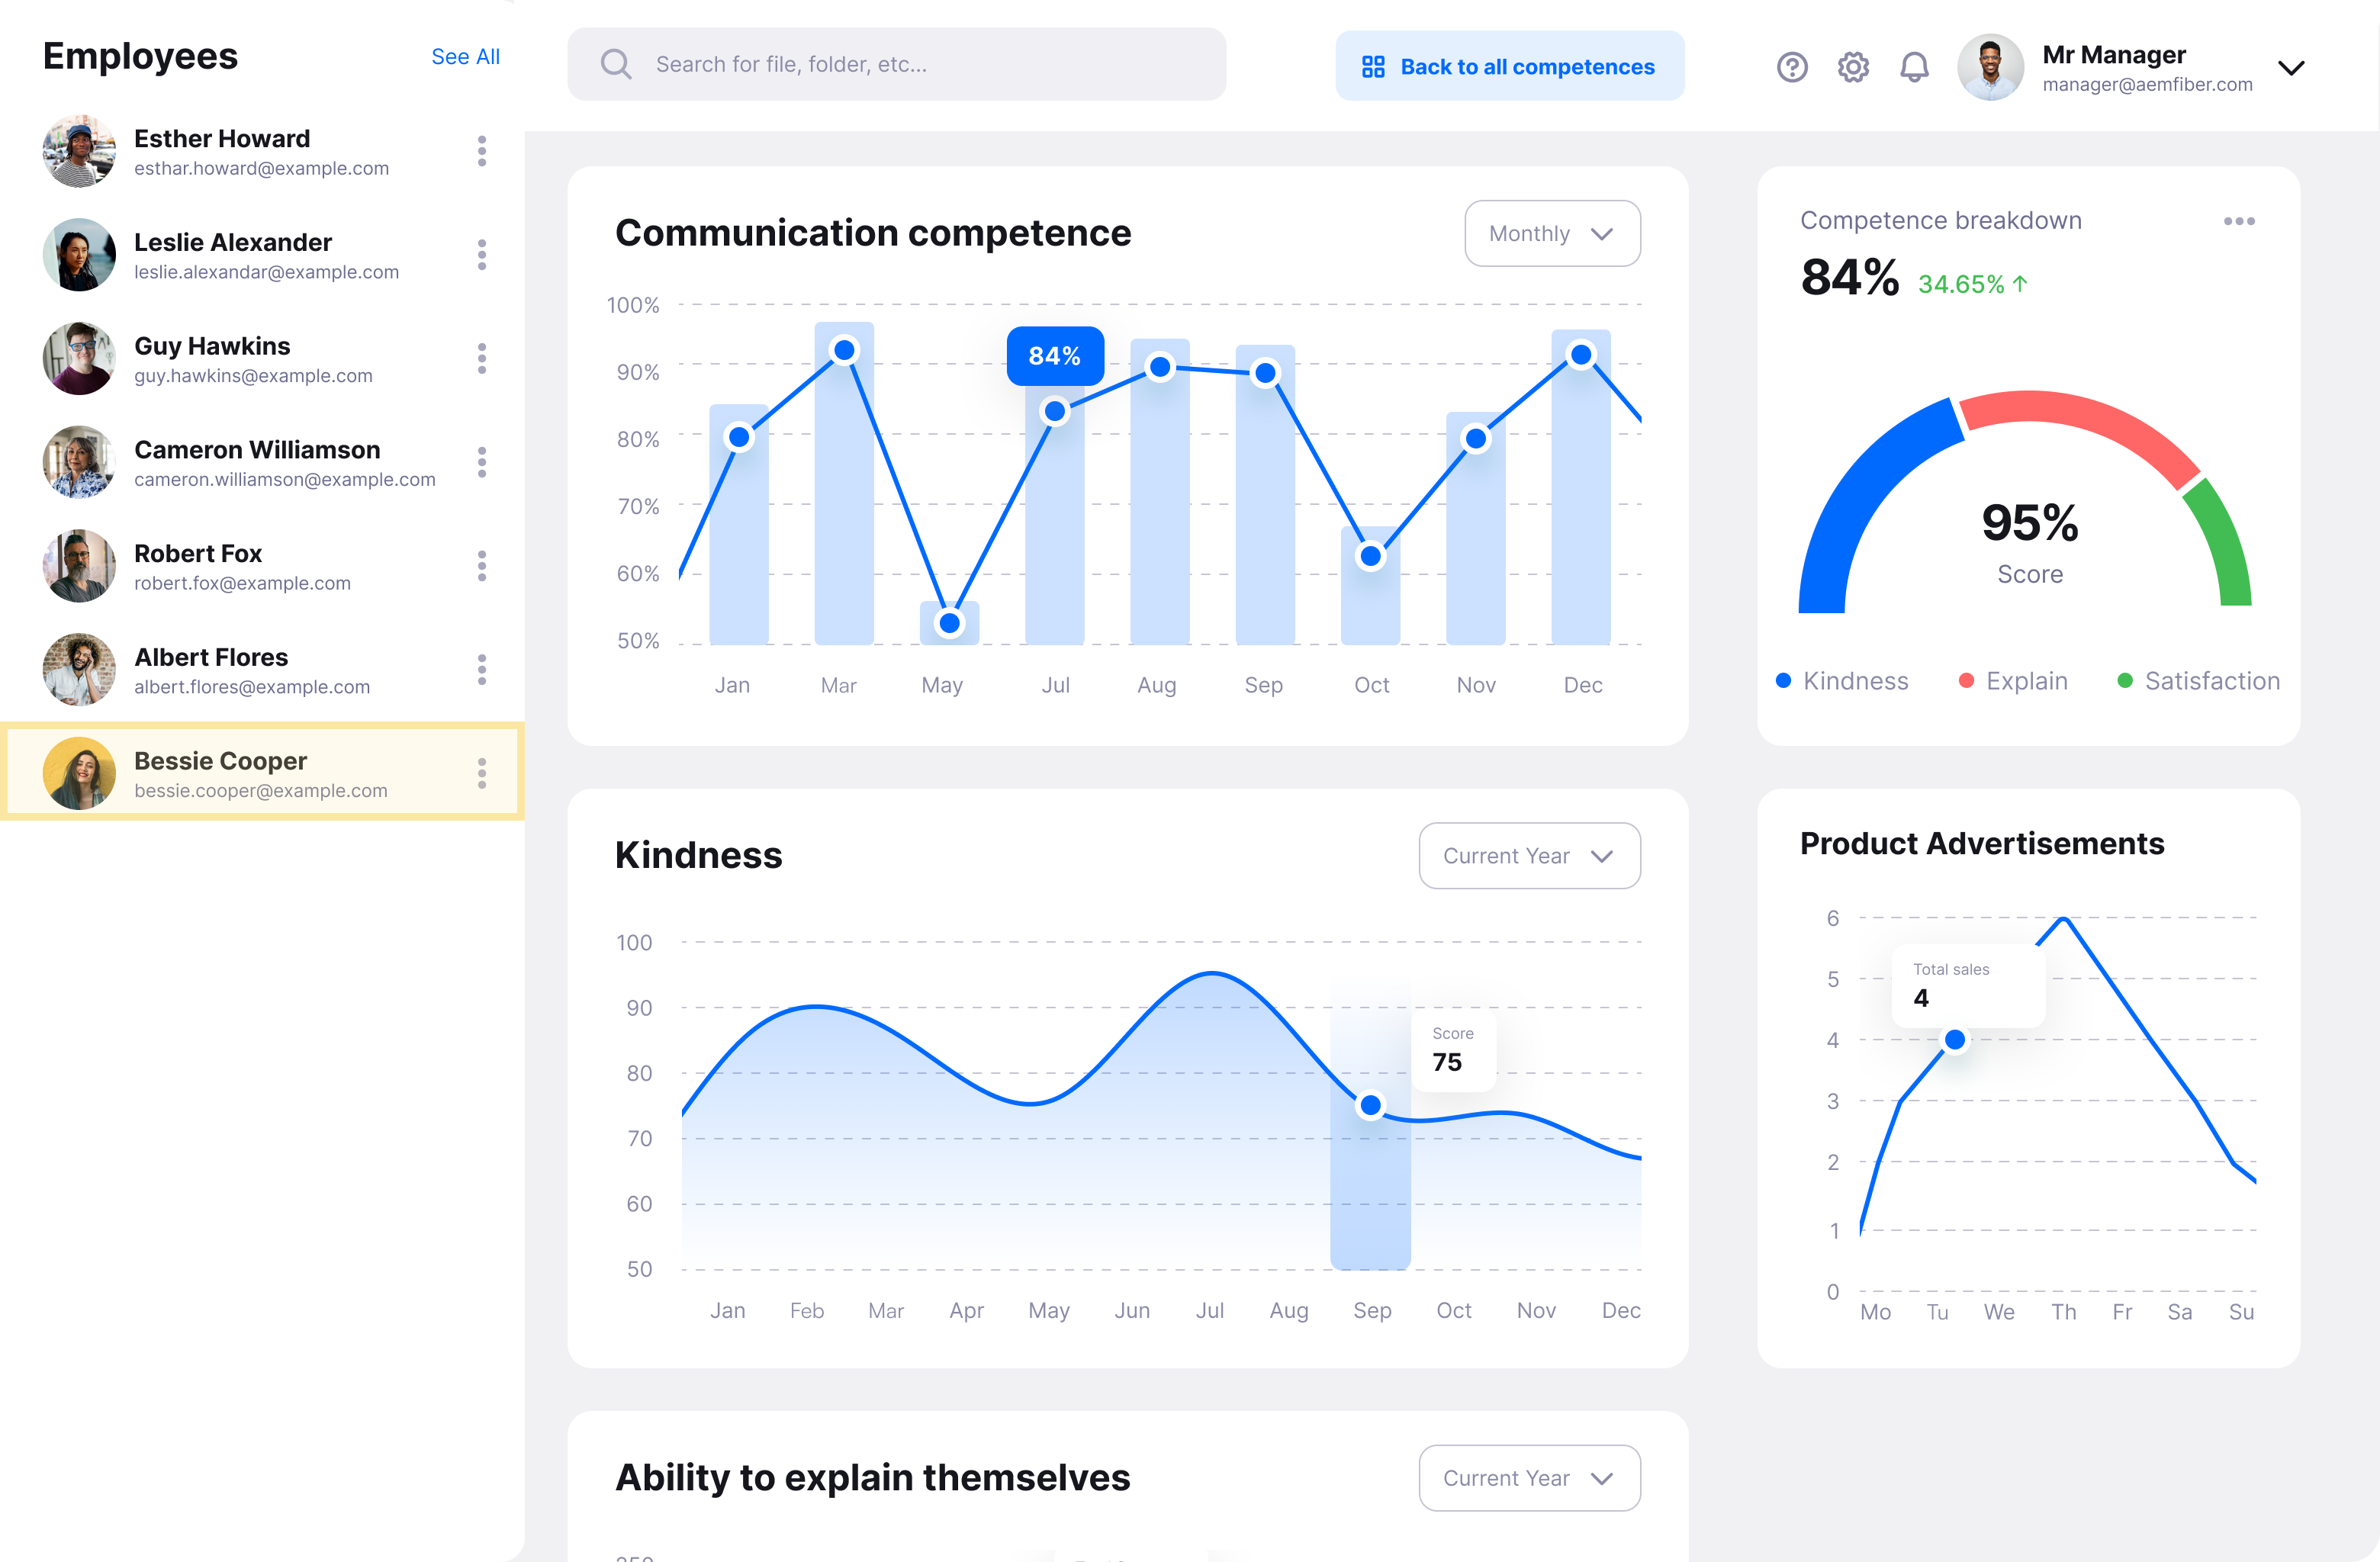
\includegraphics[width=\textwidth]{employee detail.png}
      \caption{Dashboard employee detail mock-up}
      \label{figure:employee_detail}
\end{figure}
\chapter{Conclusions}


In conclusion, this research paper has presented an examination of a subset of competences within the context of competence mapping in a telecommunication company.
In particular, we chose to test the evaluation skills of the GPT model: in summary, GPT does not excel in evaluating communication abilities and may miss some behavioral patterns. Results demonstrate the model's reliability in extracting information from text, evaluating technical proficiency, and assessing problem-solving capabilities, but its performance can vary depending on the task and data at hand. Therefore using GPT in a company's competence mapping framework should be approached with caution; at the same time, it can be particularly valuable for HR support applications. However, it is important to acknowledge that this work investigates only a fraction of the broader landscape of possible competences, and numerous aspects remain unexplored. Regarding privacy concerns, it can still be considered an issue to be discussed in a legal environment, as some of the data processed by GPT may be sensitive. As technology continues to advance, the potential for more sophisticated and capable AI models becomes increasingly evident: we believe that the new GPT-4.0, with its enhanced capabilities and deeper understanding, could serve as a valuable tool for further investigations in this domain.




\chapter{Technical Appendix}
\label{sec:techappendix}
In this technical appendix, we present an overview of the methodologies employed in our research, regarding GPT's testing phase. This supplementary section aims to provide a transparent and thorough account of the technical aspects for future reproducibility.

\section{Test Execution}
We tested the model capabilities using OpenAI's GPT API with gpt-3.5-turbo, which is the most cost-effective OpenAI model. Entering the testing phase, we had a few key expectations regarding GPT capabilities:
\begin{itemize}
      \item Sentiment Analysis. We aimed to understand if GPT could accurately determine the sentiment (positive, negative, or neutral) in a given text.
      \item Multi-option Question Answering. We aimed to evaluate GPT's ability to extract the necessary information from a text to answer multi-option questions effectively.
      \item Data Extraction. We aimed to explore how well GPT could identify and extract valuable data from both call transcriptions and working notes.
\end{itemize}
Our testing phase focused on assessing GPT's performance in these practical contexts to understand its strengths and weaknesses when applied to competence mapping tasks. Each testing phase has been divided into 4 sub-phases: Preprocess phase, Prompt construction phase, API call phase, and Results analysis phase.
\begin{enumerate}
      \item Preprocess phase. Initially, we prepared the testing data. This phase involved data cleaning and the creation of an input that the model could understand. OpenAI's best practices were followed in terms of spacing and clear distinction between different portions of the text.
      \item Prompt construction phase. During the prompt construction phase, we carefully crafted the instructions and questions intended for the model, adhering to OpenAI's guidelines to optimize the quality and efficacy of the results obtained. We made sure to specify the structure of the answer in an unequivocal way so that the model would answer in a format that allowed us to automatize the testing process.
      \item API call phase. We executed calls by transmitting the prompt to the model through the GPT3.5 API.
      \item Result analysis phase. Upon receiving the model's response, a thorough analysis of the results was conducted, and prompts were adjusted as necessary.
\end{enumerate}

\subsection{Communication competence testing}
We initiated communication competence tests to adhere to OpenAI's guidelines and best practices. The primary objective is to assess operators' ability to effectively engage with customers. We are evaluating factors such as kindness, clarity in explanations, and overall customer satisfaction with the assistance provided. Additionally, we are employing sentiment analysis to understand the emotional tone of customer-operator interactions and gauge how people feel about the support they receive. More in detail:
\begin{itemize}
      \item Kindness. The model was asked to evaluate the kindness of the operator throughout the whole conversation.
      \item Clarity in explanations. The model was tasked with assessing the operator's skill in effectively communicating information or providing explanations for potential solutions to customers' problems. This may involve guiding customers through the steps to resolve their issues or, if needed, explaining the underlying cause along with suggested solutions that the company can implement.
      \item Pitch sale execution. In the \href{https://zenodo.org/records/4274454}{I-BiDaaS TID Synthetic Call Centre Dataset}, we observed that the actor portraying the operator was frequently tasked with promoting a new product to the customer while addressing their request. To assess GPT's capability to discern the presence or absence of this scenario in the provided transcriptions, we aimed to evaluate whether the model could accurately identify instances where customer support operators deviate from established behavioral guidelines. This becomes particularly important in situations where companies have set specific guidelines for their customer support representatives and would want to understand if such guidelines are respected.
      \item Customer satisfaction. The model was asked to understand the general satisfaction of the customer.
\end{itemize}

Various prompt variants were tested, as detailed in the following section (see \ref{sec:testingresults}). In the initial approach, a single question was posed in a single prompt, asking the model to assess the operator's communication competence with a score ranging from 0 to 4. In the second approach, four distinct questions were presented in a single prompt. The model was prompted to evaluate four communication characteristics: Kindness, Ability to explain, Execution of pitch sale, and Customer satisfaction. The first, second, and fourth questions sought a value between 0 and 1 (0, 0.25, 0.5, 0.75, 1), while the third question required a binary response (0 or 1). To ensure the model focused on individual tasks, the third approach involved posing four questions in separate prompts, each requesting a response between 0 and 1 (0, 0.25, 0.5, 0.75, 1). Similarly, in the final approach, four questions were presented in separate prompts, each seeking a binary answer (0 or 1). As mentioned earlier, in response to the absence of negative behavior examples, we augmented the existing dataset by incorporating nine additional transcriptions. Each transcription is a modified version of an existing one in the original dataset, primarily focusing on creating scenarios where the operator exhibited unprofessional behavior during interactions with the customer.

\subsection{Technical competence testing}
\label{sec:techcomp}


One of the competences under evaluation is the operator's proficiency in resolving technical issues. In the case of AEM Fiber, operators are required to categorize each issue into a broad category. Our objective is to task the model with determining if the category selected by the operator aligns with the actual issue based on the ticket description. Additionally, the model is challenged to identify the sub-category associated with the ticket, aiming for a more detailed assessment of the operator's capabilities. This approach recognizes that solving similar issues in different contexts may require different solutions. In our testing, we assessed GPT's ability to accurately identify both the category and subcategory of a ticket using the ticket descriptions from the Milwaukee Dataset, with a provided list of possible categories. To model the category recognition task, where categories are very different, we selected five distinct categories from the Milwaukee Dataset. The considered categories are as follows:
\begin{itemize}
      \item 'Interior of Building in Disrepair'
      \item 'Missed Collection: Garbage'
      \item 'Pothole'
      \item 'Sanitation Inspector Notification'
      \item 'Street Light Out'
\end{itemize}
These selected categories do not overlap in any conceivable manner. To model the subcategory recognition task, we focused on the subcategories related to the "Garbage Cart" issue within the dataset. The objective is to assess the model's ability to identify very similar classes of tickets. To assist GPT in this task, we chose to provide additional information about each subcategory in the prompt. This decision is rooted in the assumption that companies like AEM Fiber possess the capacity to discern the nuances within their services, enabling them to identify the key terms that accurately distinguish each subcategory. The considered sub-categories of Garbage cart are: Additional, Damaged, Delete, and Missing.\\

To evaluate the model's ability to identify elements within the text, we tasked it with recognizing the name of the street where the issue occurred. We manually extracted the location of the problem and compared the model's response with our expected label. For this comparison, we utilized a Python package that measures the distance between two strings. If a certain threshold was surpassed, the answer was deemed correct. The package employs Levenshtein Distance to calculate differences between strings \cite{fuzzywuzzy}. For instance, in the AEM Fiber use case, this approach could prove valuable in identifying details such as the router model and manufacturer. This introduces an additional layer of information about the technical operator's capabilities, considering that different routers require distinct knowledge.

\subsection{Problem management testing}
The ultimate goal here is to evaluate the technician's problem-solving abilities, particularly in managing various client issues, described in helpdesk tickets. The operator is tasked with documenting every step of the problem management process in work notes. In our evaluation, we provided GPT with the work notes related to a ticket without explicitly specifying which ticket they corresponded to. Subsequently, we assessed GPT's capacity to accurately identify if the notes adhered to the guidelines established by domain experts. For example, if a ticket needs to be resolved within two days, we asked GPT to analyze the work notes to determine if the tickets were appropriately resolved within 48 hours. Additionally, considering the significance of keeping the client continuously updated during the ticket resolution process, we tasked GPT with identifying if this requirement was met by the technician. The complete list of requests made to GPT is available in section \ref{sec:probmanageres}. Each question includes a set of possible answers, and we assigned a specific score to each answer. In the initial test phase, we initially asked GPT all these questions in a single call. However, we observed improved performance when each question corresponded to a single query. For each group of notes related to a ticket, we manually determined the expected scores and then compared them with the scores given by GPT.

\section{Testing Results}
\label{sec:testingresults}

We will now provide an example of the structure used for each prompt. Initially, we described to the model the provided text format and content. Occasionally we also told GPT to assume the role of a persona following the OpenAI best practices.
\begin{center}
      \textit{You need to evaluate the following conversation between a customer and an operator, contained in a list. Each sentence in the list is separated by a comma and starts with an identifier that reveals who is speaking (Either 'Customer' or 'Tech'). You are a Human Resources employee and you have to answer the following question:}
\end{center}
We then added a question to the prompt.
\begin{center}
      \textit{Is the number of days it took to resolve the issue greater than 2? Yes: -1; No: +1.}
\end{center}
We also provided the model with examples and additional information regarding each competence and finally we explained to the model which rating scale to use and the answer structure.
\begin{center}
      \textit{Give me 1 if the operator was professional, 0 otherwise. You have to answer only with the score for each question.}
\end{center}
We considered appropriate the choice of the Root Mean Square Error (RMSE) as the metric for measuring GPT's error, especially given its effectiveness in quantifying the accuracy of predictions in regression problems. The RMSE provides a comprehensive evaluation of the differences between predicted and actual values, making it a suitable metric for assessing GPT's performance in this context. Specifically, the RMSE is calculated by computing the difference between the target value \(\hat{y_i}\) and the GPT predicted value \(y_i\).
\begin{center}
      \[ RMSE: \sqrt{ \frac{1}{n}\sum_{i=1}^n (\hat{y_i} - y_i)^2}\]
\end{center}

\section{Communication Results}

\subsection{Version 1.0}
The prompt was structured as described before. The following is the version-specific question:\\

\textit{How good was the communication competence of the tech operator?}\\

The following are the obtained results:\\
\begin{center}
      \begin{tabular}{cccc}
            \toprule
            Transcription number (\#) & Overall (OV) & Target Overall (TOV) & Difference \\
            \midrule
            1                         & 4            & 4                    & 0          \\
            2                         & 4            & 4                    & 0          \\
            3                         & 4            & 4                    & 0          \\
            4                         & 4            & 4                    & 0          \\
            5                         & 4            & 4                    & 0          \\
            6                         & 4            & 3                    & -1         \\
            7                         & 4            & 4                    & 0          \\
            8                         & 4            & 4                    & 0          \\
            9                         & 4            & 4                    & 0          \\
            10                        & 4            & 3                    & -1         \\
            11                        & 2            & 2                    & 0          \\
            12                        & 1            & 0                    & -1         \\
            13                        & 2            & 1                    & -1         \\
            14                        & 1            & 1                    & 0          \\
            15                        & 0            & 0                    & 0          \\
            16                        & 4            & 2                    & -2         \\
            17                        & 1            & 0                    & -1         \\
            18                        & 0            & 0                    & 0          \\
            \bottomrule
      \end{tabular}

\end{center}

\subsection{Version 1.1}
The prompt was structured as described before. The questions are the same as in the previous version. The following are the obtained results:
\begin{center}
      \begin{tabular}{ccccccccccccc}
            \toprule
            \# & KIND & EXP & SALE & SAT & TKIND & TEXP & TSALE & TSAT & OV & TOV & DIFF \\

            \midrule
            1  & 1    & 1   & 1    & 1   & 1     & 1    & 1     & 1    & 4  & 4   & 0    \\
            2  & 1    & 1   & 1    & 1   & 1     & 1    & 1     & 1    & 4  & 4   & 0    \\
            3  & 1    & 1   & 1    & 1   & 1     & 1    & 1     & 1    & 4  & 4   & 0    \\
            4  & 1    & 1   & 1    & 1   & 1     & 1    & 1     & 1    & 4  & 4   & 0    \\
            5  & 1    & 1   & 1    & 1   & 1     & 1    & 1     & 1    & 4  & 4   & 0    \\
            6  & 1    & 1   & 1    & 1   & 1     & 1    & 0     & 1    & 4  & 3   & -1   \\
            7  & 1    & 1   & 1    & 1   & 1     & 1    & 1     & 1    & 4  & 4   & 0    \\
            8  & 1    & 1   & 1    & 1   & 1     & 1    & 1     & 1    & 4  & 4   & 0    \\
            9  & 1    & 1   & 1    & 1   & 1     & 1    & 1     & 1    & 4  & 4   & 0    \\
            10 & 1    & 1   & 0    & 1   & 1     & 1    & 0     & 1    & 3  & 3   & 0    \\
            11 & 0    & 0   & 1    & 0   & 0     & 1    & 1     & 0    & 1  & 2   & 1    \\
            12 & 0    & 0   & 0    & 0   & 0     & 0    & 0     & 0    & 0  & 0   & 0    \\
            13 & 0    & 0   & 0    & 0   & 0     & 0    & 0     & 0    & 0  & 0   & 0    \\
            14 & 0    & 0   & 0    & 0   & 0     & 0    & 0     & 0    & 0  & 0   & 0    \\
            15 & 0    & 0   & 0    & 0   & 0     & 0    & 0     & 0    & 0  & 0   & 0    \\
            16 & 1    & 1   & 1    & 1   & 1     & 1    & 1     & 0    & 4  & 3   & -1   \\
            17 & 0    & 0   & 0    & 0   & 0     & 0    & 0     & 0    & 0  & 0   & 0    \\
            18 & 0    & 0   & 0    & 0   & 0     & 0    & 0     & 0    & 0  & 0   & 0    \\
            \bottomrule
      \end{tabular}
\end{center}

\subsection{Version 2.0}
The prompt was structured as described before. The following are the version specific questions:\\

\textit{Was the tech operator kind?\\
      Was the tech operator able to explain himself?\\
      Was the tech operator able to mention the existence of additional products while conversating with the customer?\\
      Was the customer satisfied with the tech service in the end?
}\\

The following are the obtained results:\\
\begin{center}
      \begin{tabular}{ccccccccccccc}
            \toprule
            \# & KIND & EXP  & SALE & SAT  & TKIND & TEXP & TSALE & TSAT & OV   & TOV  & DIFF  \\
            \midrule
            1  & 0.75 & 1.00 & 1    & 0.75 & 1.00  & 1.00 & 1     & 1.00 & 3.50 & 4.00 & 0.50  \\
            2  & 0.75 & 1.00 & 1    & 1.00 & 1.00  & 0.75 & 1     & 1.00 & 3.75 & 3.75 & 0.00  \\
            3  & 0.75 & 1.00 & 1    & 0.75 & 1.00  & 0.75 & 1     & 1.00 & 3.50 & 3.75 & 0.25  \\
            4  & 0.75 & 1.00 & 1    & 0.75 & 1.00  & 0.75 & 1     & 1.00 & 3.50 & 3.75 & 0.25  \\
            5  & 0.75 & 1.00 & 1    & 0.75 & 1.00  & 1.00 & 1     & 1.00 & 3.50 & 4.00 & 0.50  \\
            6  & 0.75 & 1.00 & 0    & 0.75 & 1.00  & 0.75 & 0     & 0.75 & 2.50 & 2.50 & 0.00  \\
            7  & 0.75 & 0.75 & 1    & 0.75 & 1.00  & 1.00 & 1     & 1.00 & 3.25 & 4.00 & 0.75  \\
            8  & 0.75 & 1.00 & 1    & 0.75 & 1.00  & 1.00 & 1     & 1.00 & 3.50 & 4.00 & 0.50  \\
            9  & 0.75 & 1.00 & 1    & 1.00 & 1.00  & 1.00 & 1     & 1.00 & 3.75 & 4.00 & 0.25  \\
            10 & 0.75 & 0.75 & 0    & 0.75 & 1.00  & 1.00 & 0     & 1.00 & 2.25 & 3.00 & 0.75  \\
            11 & 0.75 & 0.75 & 1    & 0.75 & 0.00  & 1.00 & 1     & 0.00 & 3.25 & 2.00 & -1.25 \\
            12 & 0.75 & 0.75 & 0    & 0.50 & 0.00  & 0.00 & 0     & 0.00 & 2.00 & 0.00 & -2.00 \\
            13 & 0.75 & 0.75 & 0    & 0.75 & 0.00  & 0.50 & 0     & 0.00 & 2.25 & 0.50 & -1.75 \\
            14 & 0.75 & 1.00 & 0    & 0.25 & 0.00  & 0.50 & 0     & 0.00 & 2.00 & 0.50 & -1.50 \\
            15 & 0.00 & 0.00 & 0    & 0.00 & 0.00  & 0.00 & 0     & 0.00 & 0.00 & 0.00 & 0.00  \\
            16 & 0.75 & 1.00 & 0    & 0.75 & 0.75  & 1.00 & 1     & 0.50 & 2.50 & 3.25 & 0.75  \\
            17 & 0.75 & 0.75 & 0    & 0.25 & 0.00  & 0.00 & 0     & 0.00 & 1.75 & 0.00 & -1.75 \\
            18 & 0.00 & 0.25 & 0    & 0.00 & 0.00  & 0.00 & 0     & 0.00 & 0.25 & 0.00 & -0.25 \\
            \bottomrule
      \end{tabular}
\end{center}

\subsection{Version 2.1}
The prompt was structured as described before. The questions are the same as in the previous version. The following are the obtained results:
\begin{center}
      \begin{tabular}{ccccccccccccc}
            \toprule
            \# & KIND & EXP & SALE & SAT & TKIND & TEXP & TSALE & TSAT & OV & TOV  & DIFF  \\

            \midrule
            1  & 1    & 1   & 1    & 1   & 1.00  & 1.00 & 1     & 1.00 & 4  & 4.00 & 0.00  \\
            2  & 1    & 1   & 1    & 1   & 1.00  & 0.75 & 1     & 1.00 & 4  & 3.75 & -0.25 \\
            3  & 1    & 1   & 1    & 1   & 1.00  & 0.75 & 1     & 1.00 & 4  & 3.75 & -0.25 \\
            4  & 1    & 1   & 1    & 1   & 1.00  & 0.75 & 1     & 1.00 & 4  & 3.75 & -0.25 \\
            5  & 1    & 1   & 1    & 1   & 1.00  & 1.00 & 1     & 1.00 & 4  & 4.00 & 0.00  \\
            6  & 1    & 1   & 1    & 1   & 1.00  & 0.75 & 0     & 0.75 & 4  & 2.50 & -1.50 \\
            7  & 1    & 1   & 1    & 1   & 1.00  & 1.00 & 1     & 1.00 & 4  & 4.00 & 0.00  \\
            8  & 1    & 1   & 1    & 1   & 1.00  & 1.00 & 1     & 1.00 & 4  & 4.00 & 0.00  \\
            9  & 1    & 1   & 1    & 1   & 1.00  & 1.00 & 1     & 1.00 & 4  & 4.00 & 0.00  \\
            10 & 1    & 1   & 0    & 1   & 1.00  & 1.00 & 0     & 1.00 & 3  & 3.00 & 0.00  \\
            11 & 1    & 1   & 1    & 1   & 0.00  & 1.00 & 1     & 0.00 & 4  & 2.00 & -2.00 \\
            12 & 0    & 1   & 0    & 1   & 0.00  & 0.00 & 0     & 0.00 & 2  & 0.00 & -2.00 \\
            13 & 1    & 1   & 0    & 1   & 0.00  & 0.50 & 0     & 0.00 & 3  & 0.50 & -2.50 \\
            14 & 0    & 1   & 0    & 1   & 0.00  & 0.50 & 0     & 0.00 & 2  & 0.50 & -1.50 \\
            15 & 0    & 0   & 0    & 0   & 0.00  & 0.00 & 0     & 0.00 & 0  & 0.00 & 0.00  \\
            16 & 1    & 1   & 1    & 1   & 0.75  & 1.00 & 1     & 0.50 & 4  & 3.25 & -0.75 \\
            17 & 0    & 0   & 0    & 0   & 0.00  & 0.00 & 0     & 0.00 & 0  & 0.00 & 0.00  \\
            18 & 0    & 0   & 0    & 0   & 0.00  & 0.00 & 0     & 0.00 & 0  & 0.00 & 0.00  \\
            \bottomrule
      \end{tabular}
\end{center}

\subsection{Communication results comparison}
The RMSE was calculated for each version. Both the overall value and each single indicator have been analyzed.
\begin{center}
      \begin{figure}[ht]
            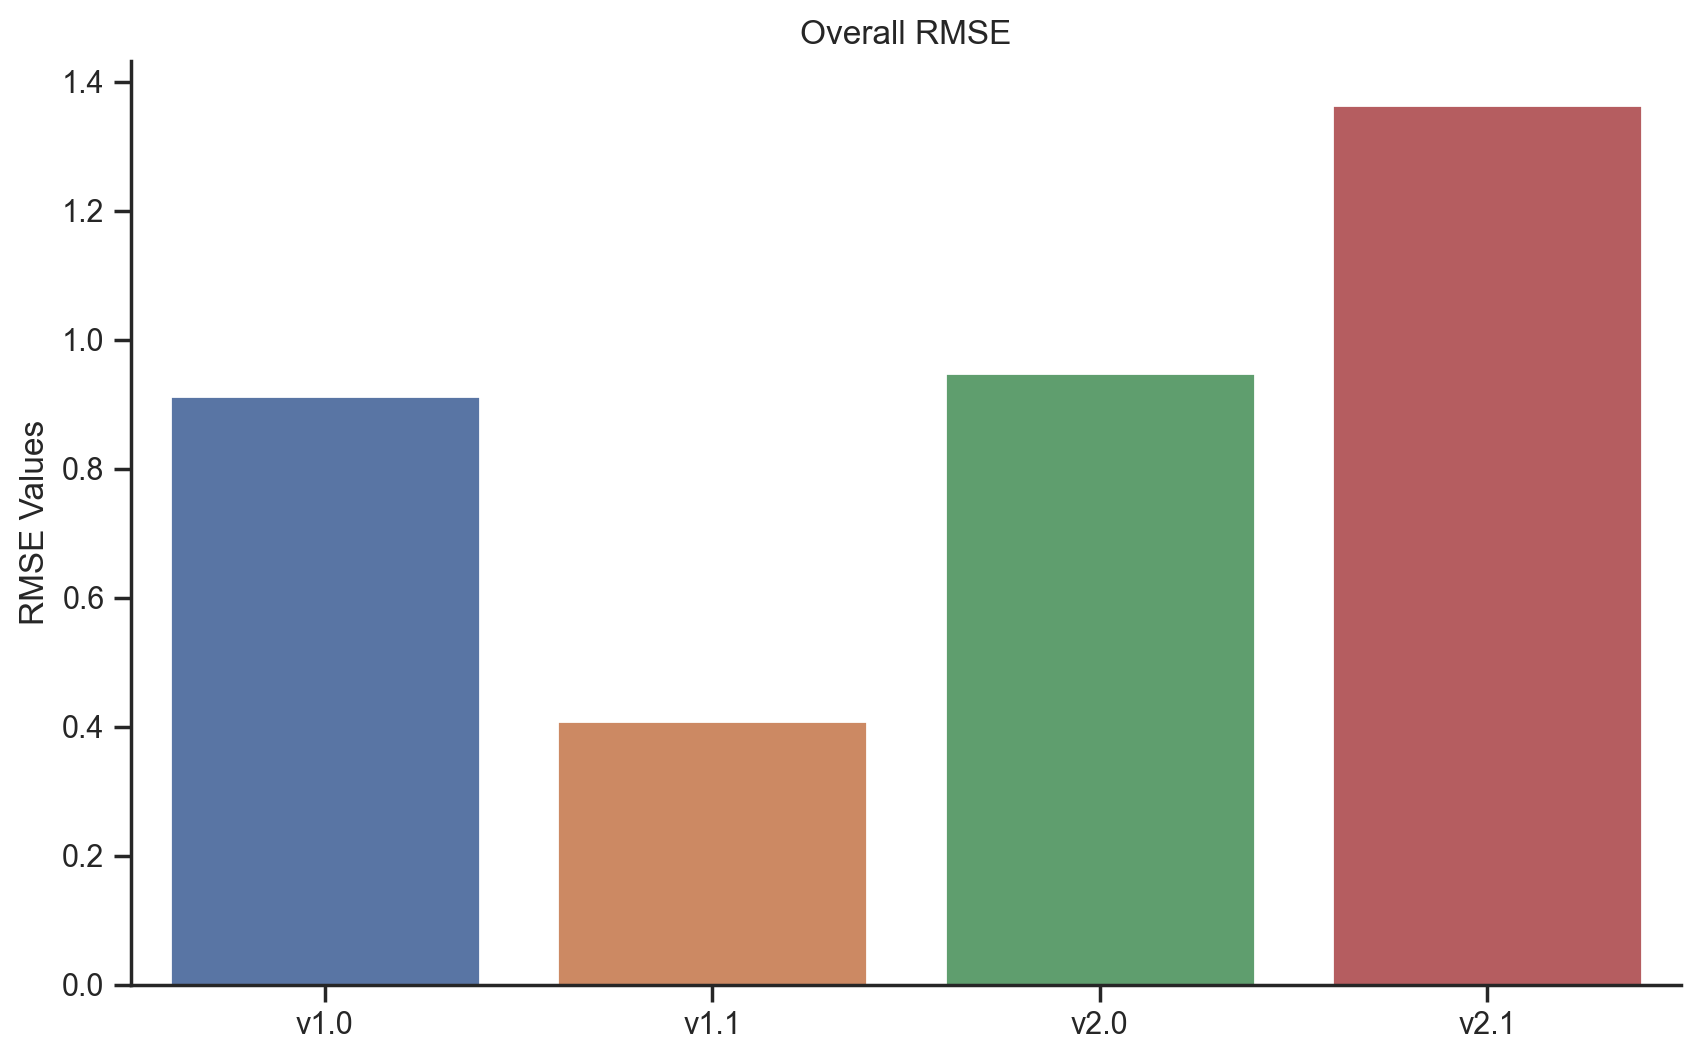
\includegraphics[width=\textwidth]{barplot_overall_score.png}
      \end{figure}
\end{center}
As we can see in the graph, version 1.0 has an RMSE of 0.912. Version 2.0 instead has an RMSE of 0.948. Version 2.1 is the worst one with an RMSE of 1.36. Version 1.1 is the best-performing one with an RMSE of 0.408.
The first approach (1.0) is good in terms of RMSE but not very informative as it only gives a broad evaluation of the operator's communication capabilities, without investigating in detail which are their strengths and weaknesses. The best version in terms of RMSE is 1.1, which also gives a more detailed view of the operator's skills. In the second approach (2.*) the information is more granular, but neither 2.0 nor 2.1 is good enough in terms of RMSE.
\begin{center}
      \begin{figure}
            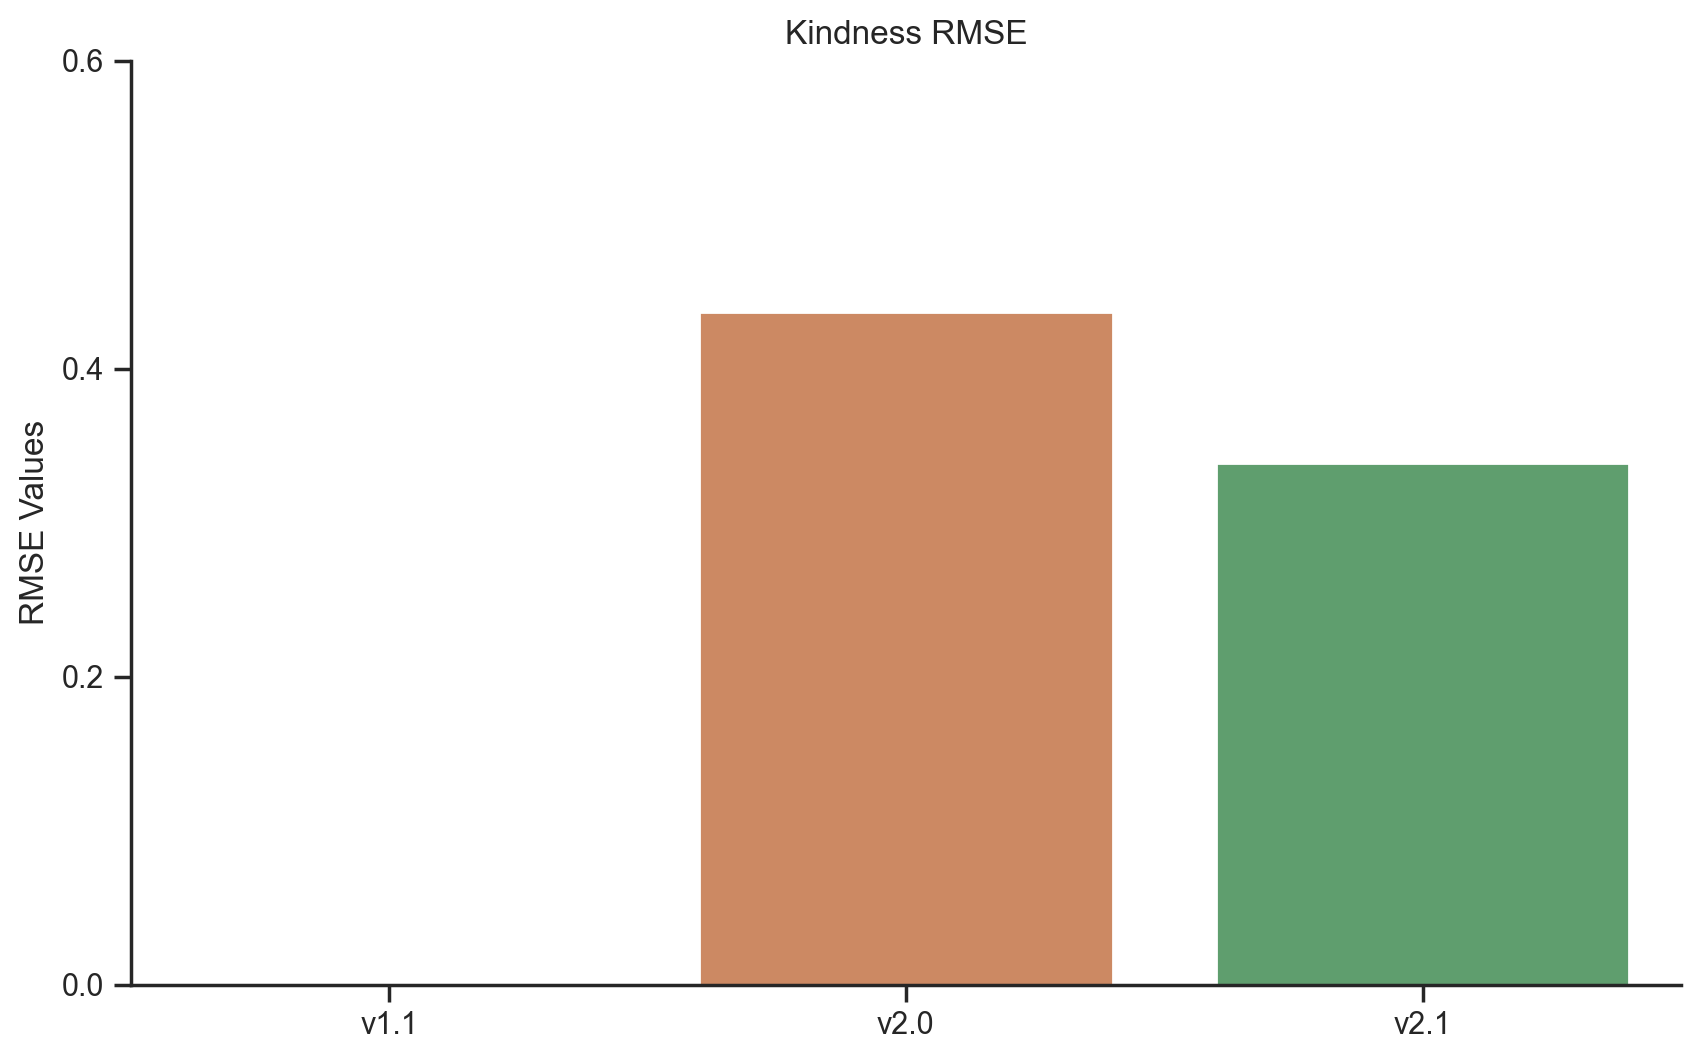
\includegraphics[width=\textwidth]{kindness_score.png}
            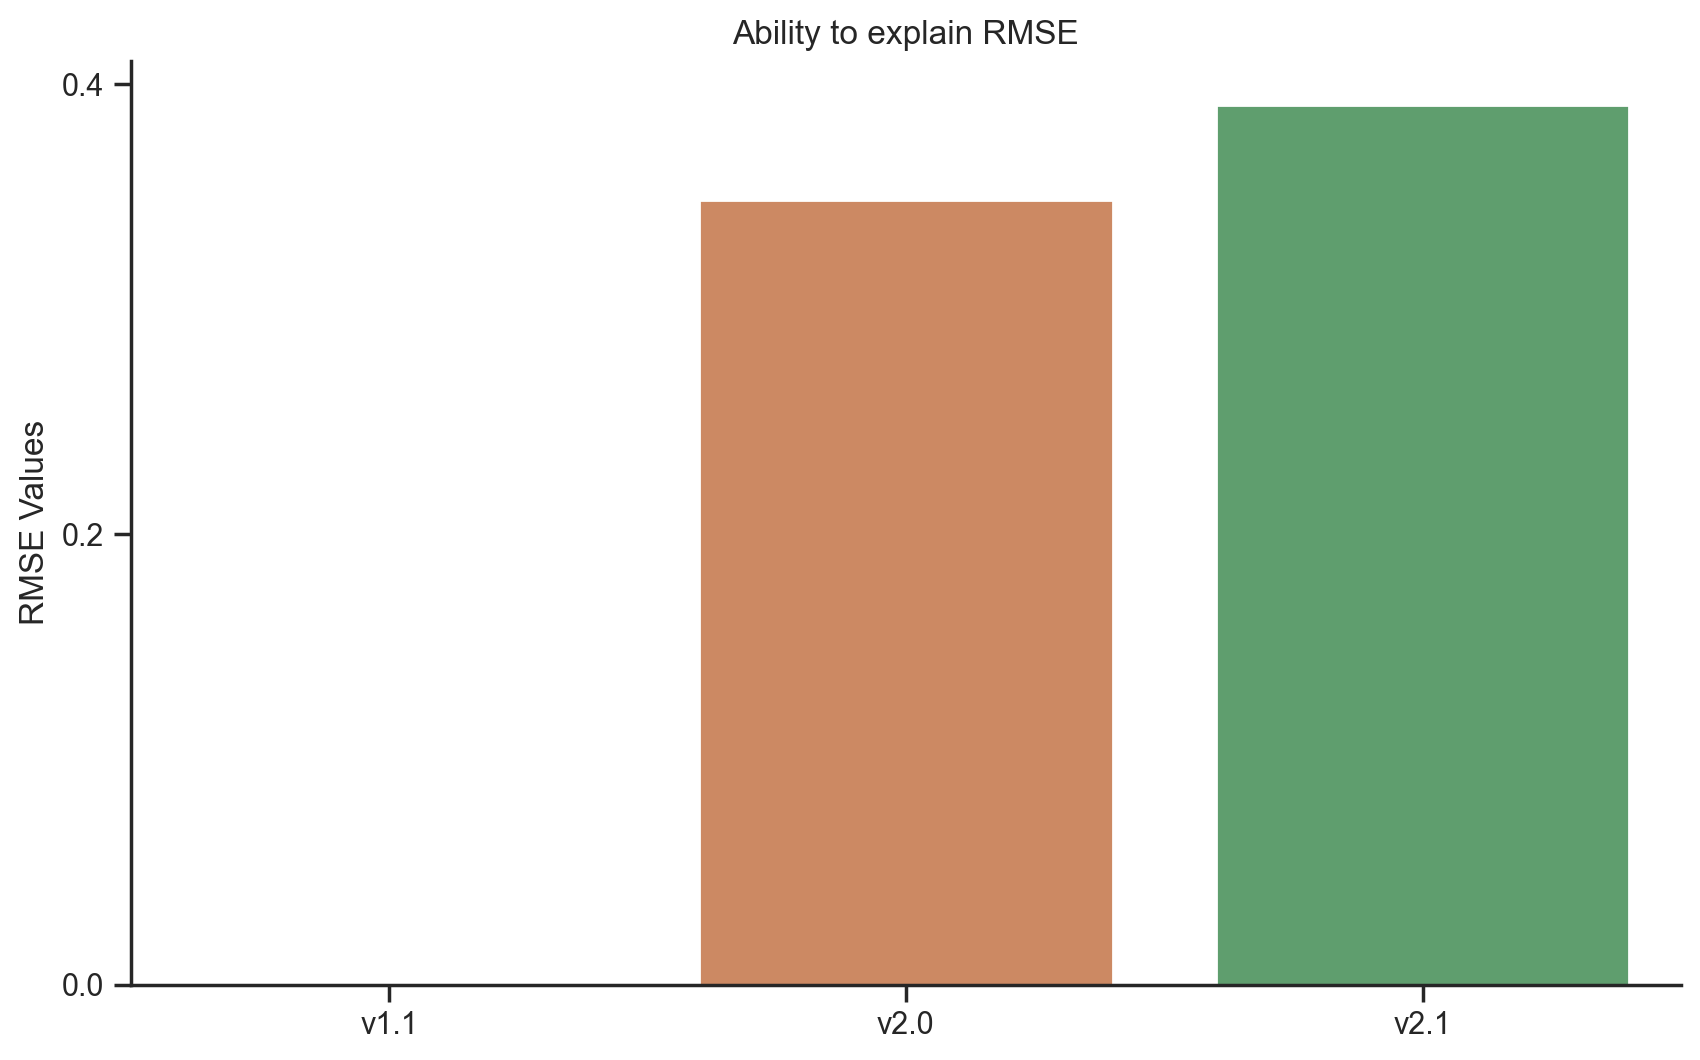
\includegraphics[width=\textwidth]{ate_score.png}
      \end{figure}
      \begin{figure}
            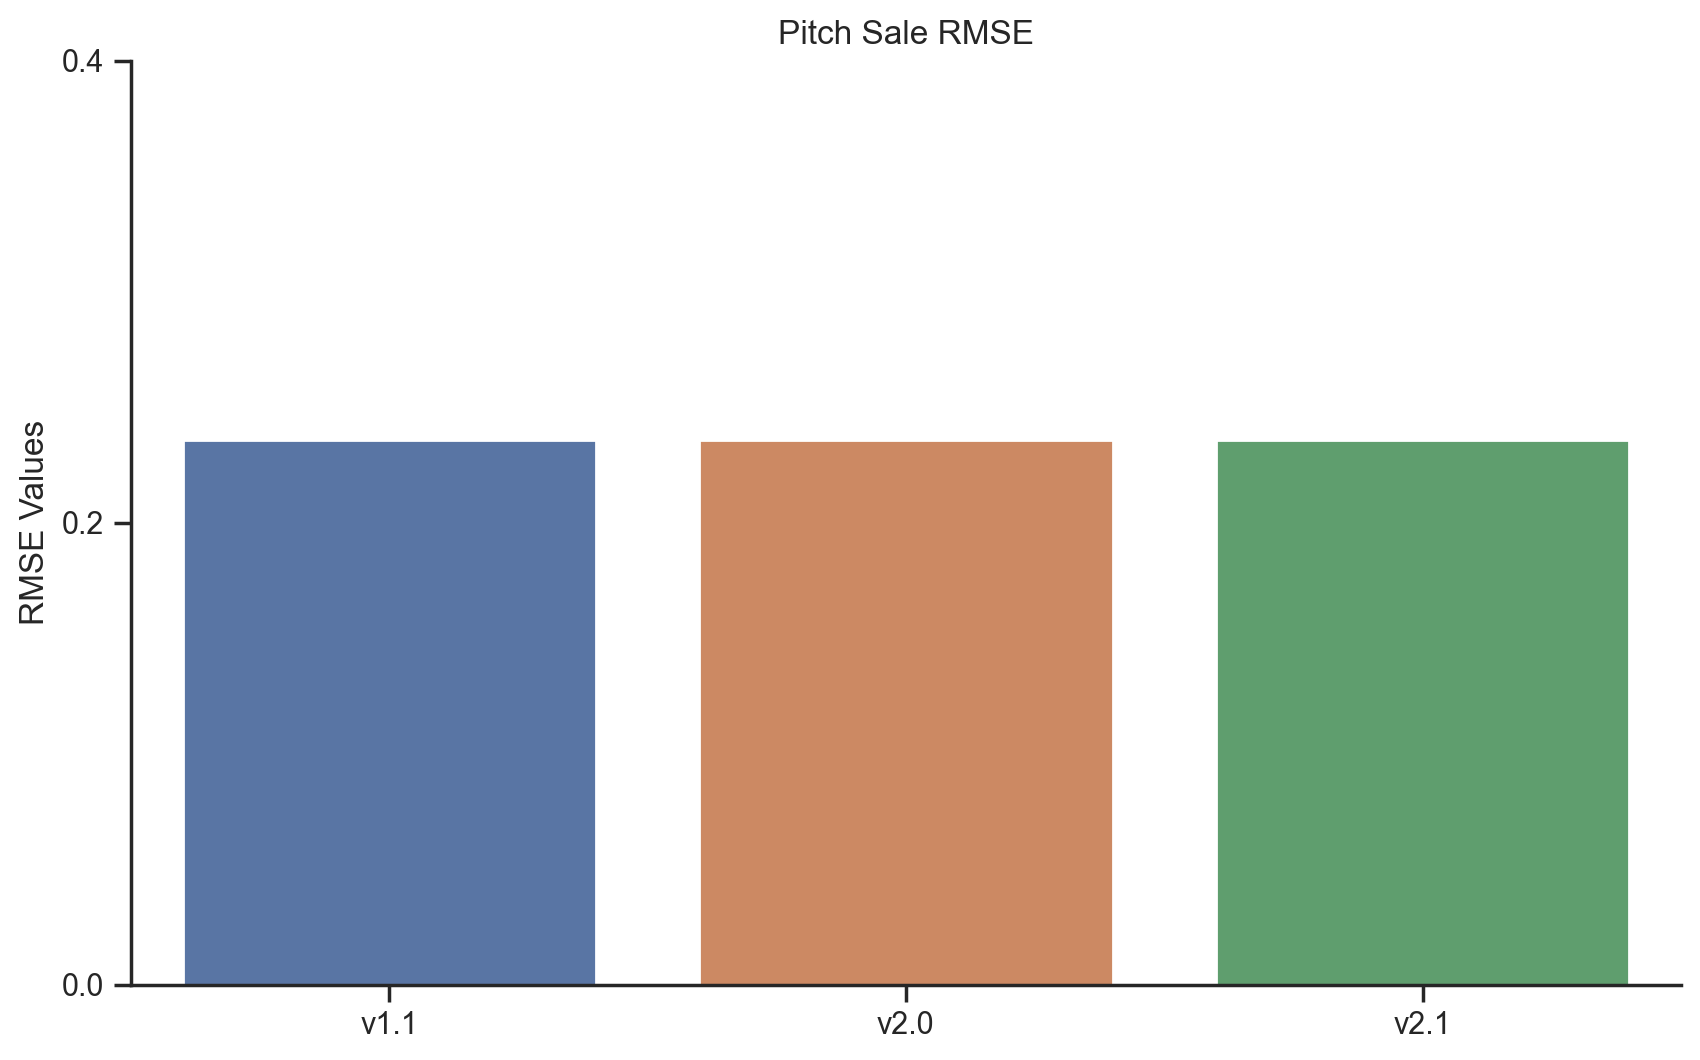
\includegraphics[width=\textwidth]{ps_score.png}
            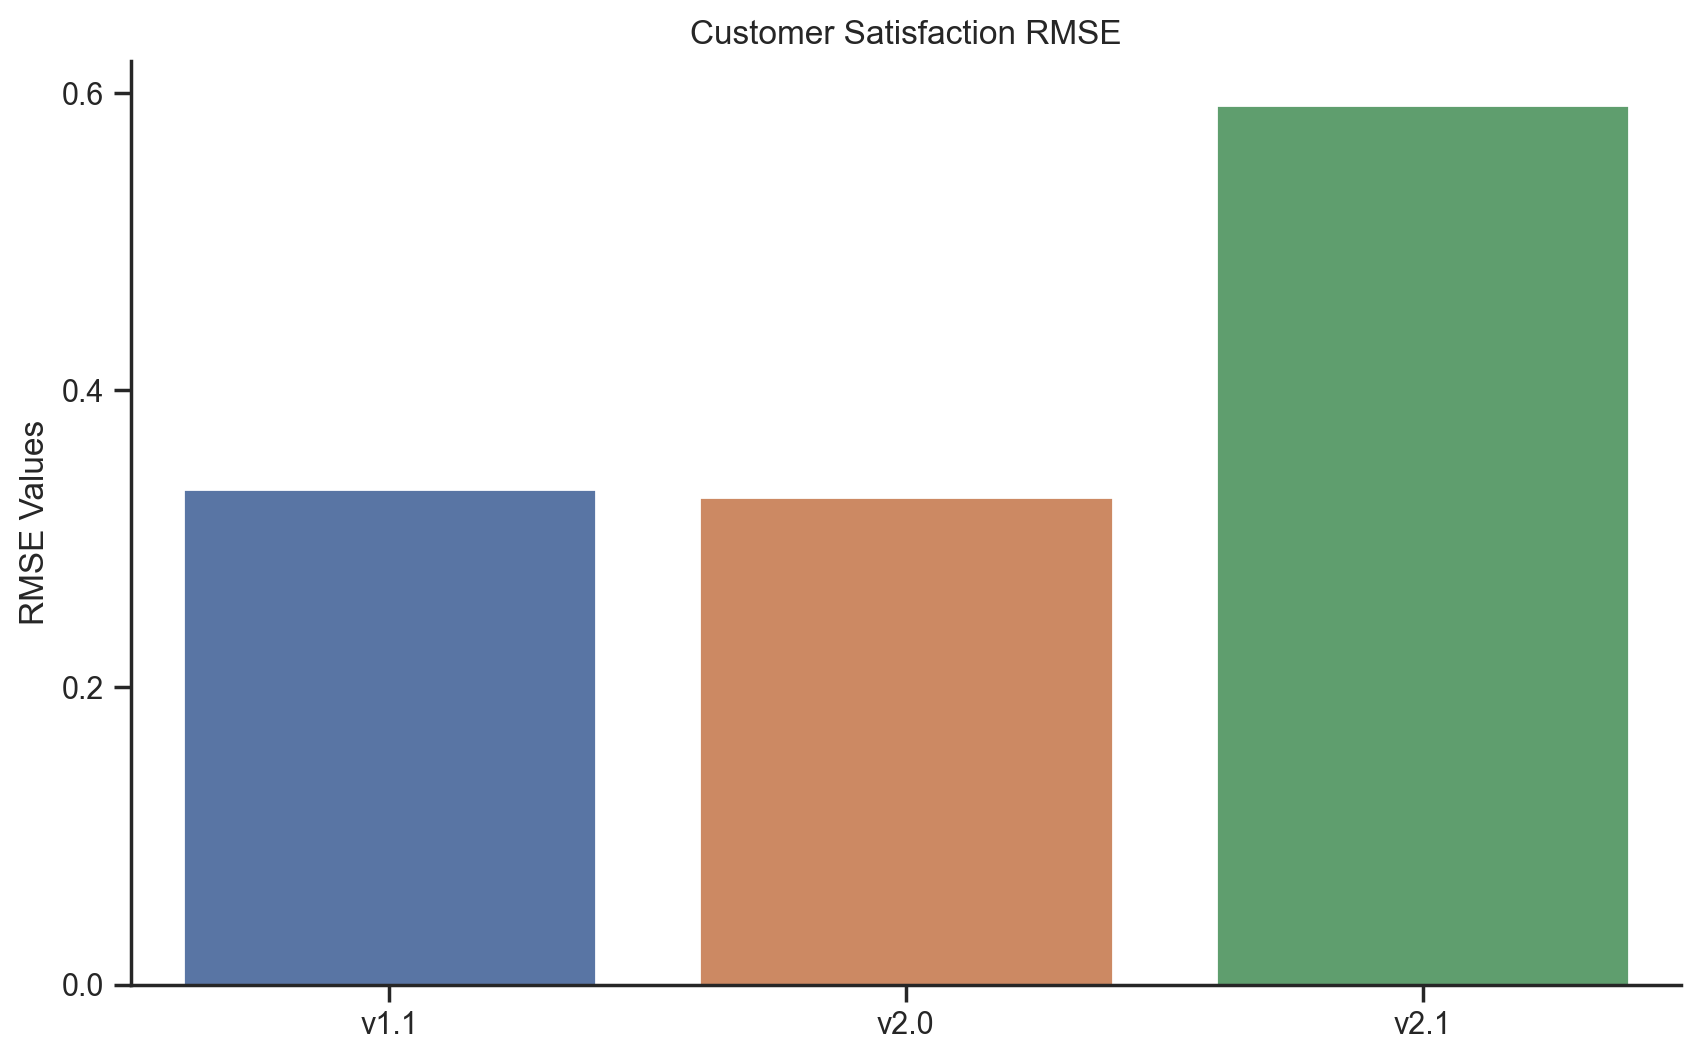
\includegraphics[width=\textwidth]{cs_score.png}
      \end{figure}
\end{center}
As expected, the error on single sub-scores reflects the error on the overall score. It's worth noting that the Pitch Sale sub-score is equal for all the versions evaluating skills separately.
\begin{center}
      \begin{figure}[ht]
            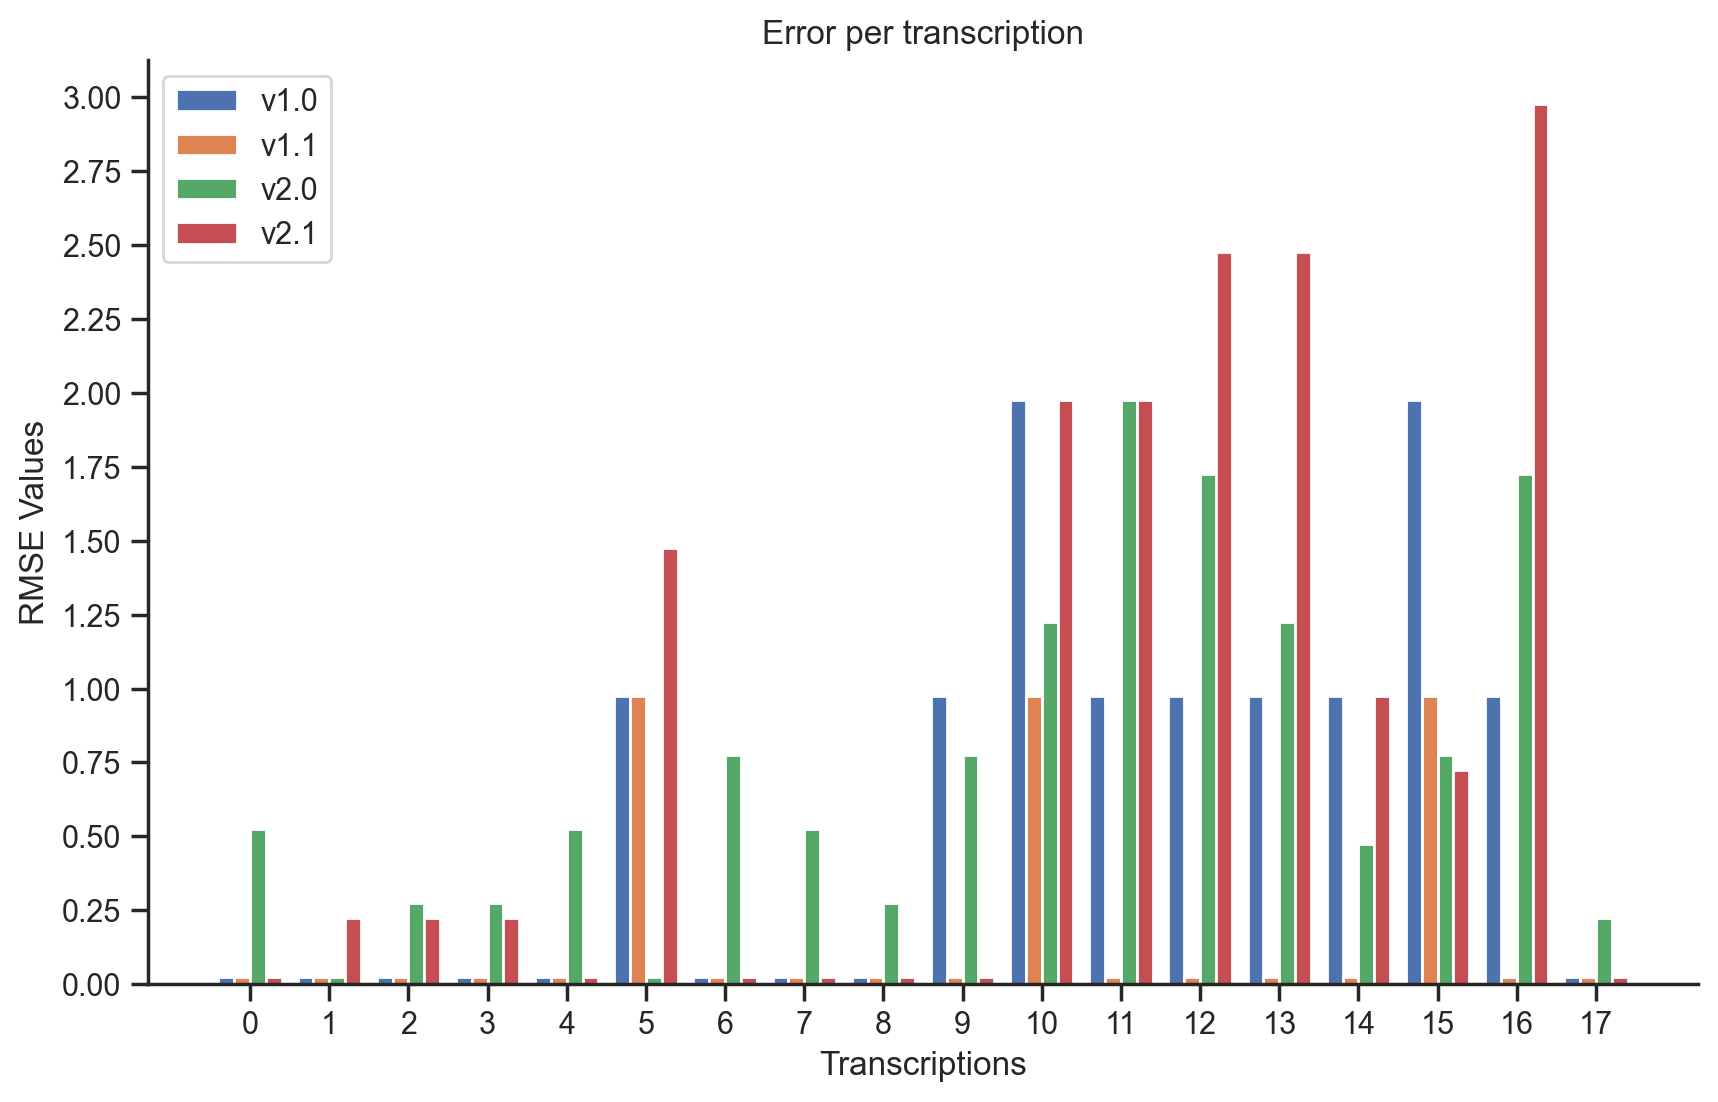
\includegraphics[width=\textwidth]{error_per_transcription.png}
      \end{figure}
\end{center}

It's notable that a significant proportion of errors occur in the additional transcriptions, particularly those that were modified to include instances of unprofessional behavior by the operator. This observation suggests that the introduction of scenarios with unprofessional behavior poses a greater challenge for accurate model performance. It's worth noting that GPT may not be entirely reliable in an automated communication competence mapping context, and caution is warranted when considering its use in a fully automated scoring framework. However, recognizing its potential as a supportive tool for HR purposes is a constructive approach. Leveraging GPT as an assistive tool, rather than relying on it solely for automated decisions, allows human judgment to complement and refine the outputs, contributing to a more nuanced and accurate evaluation process.

\section{Technical Skill Results}

\subsection{Categories and Streets}
The prompt was structured as described before. The following is the version specific question:\\

\textit{Can you identify the category of the ticket and the street in which the problem occurred?}\\

The following are the obtained results:
\begin{center}
      \begin{tabular}{lllrllr}
            \toprule
            \# & CAT       & TCAT      & ICC  & TSTREET       & STREET         & STRSCORE \\
            \midrule
            0  & Disrepair & Disrepair & True & 23rd Street   & 23rd Street    & 100      \\
            1  & Disrepair & Disrepair & True & Atkinson Ave  & W Atkinson Ave & 92       \\
            2  & Disrepair & Disrepair & True & Alvina Ave    & 0              & 0        \\
            3  & Disrepair & Disrepair & True & 0             & 0              & 100      \\
            4  & Disrepair & Disrepair & True & 0             & 0              & 100      \\
            5  & Disrepair & Disrepair & True & 0             & 0              & 100      \\
            6  & Disrepair & Disrepair & True & 0             & 0              & 100      \\
            7  & Disrepair & Disrepair & True & 0             & 0              & 100      \\
            8  & Disrepair & Disrepair & True & 85th Street   & 85th St        & 78       \\
            9  & Disrepair & Disrepair & True & 0             & 0              & 100      \\
            10 & Disrepair & Disrepair & True & 33rd Street   & 33RD ST        & 78       \\
            11 & Disrepair & Disrepair & True & 0             & 0              & 100      \\
            85 & Pothole   & Pothole   & True & 69th Street   & 69th Street    & 100      \\
            86 & Pothole   & Pothole   & True & Rohr Ave      & Rohr Av        & 93       \\
            87 & Pothole   & Pothole   & True & 80th Street   & 80th Street    & 100      \\
            88 & Pothole   & Pothole   & True & 61st Street   & 61st St.       & 74       \\
            90 & Pothole   & Pothole   & True & mason Street  & E Mason Street & 92       \\
            91 & Pothole   & Pothole   & True & 40th Street   & N. 40th St.    & 80       \\
            92 & Pothole   & Pothole   & True & Howard Ave    & E Howard Ave   & 91       \\
            93 & Pothole   & Pothole   & True & Harbor Street & Harbor Street  & 100      \\
            \bottomrule
      \end{tabular}
\end{center}

\subsection{Subcategories}
The prompt was structured as described before. The following is the version specific question:\\

\textit{The problems are related to previously identified category. Can you identify the ticket subcategory?}\\

The following are the obtained results:
\begin{center}
      \begin{tabular}{lllr}
            \toprule
            \# & SUBC                     & TSUBC                    & ISC   \\
            \midrule
            0  & Garbage Cart: Additional & Garbage Cart: Additional & True  \\
            1  & Garbage Cart: Additional & Garbage Cart: Additional & True  \\
            2  & Garbage Cart: Additional & Garbage Cart: Additional & True  \\
            3  & Garbage Cart: Missing    & Garbage Cart: Additional & False \\
            4  & Garbage Cart: Additional & Garbage Cart: Additional & True  \\
            5  & Garbage Cart: Additional & Garbage Cart: Additional & True  \\
            6  & Garbage Cart: Damaged    & Garbage Cart: Additional & False \\
            7  & Garbage Cart: Additional & Garbage Cart: Additional & True  \\
            8  & Garbage Cart: Damaged    & Garbage Cart: Additional & False \\
            9  & Garbage Cart: Additional & Garbage Cart: Additional & True  \\
            10 & Garbage Cart: Additional & Garbage Cart: Additional & True  \\
            11 & Garbage Cart: Additional & Garbage Cart: Additional & True  \\
            12 & Garbage Cart: Additional & Garbage Cart: Additional & True  \\
            13 & Garbage Cart: Additional & Garbage Cart: Additional & True  \\
            14 & Garbage Cart: Additional & Garbage Cart: Additional & True  \\
            15 & Garbage Cart: Additional & Garbage Cart: Additional & True  \\
            16 & Garbage Cart: Additional & Garbage Cart: Additional & True  \\
            17 & Garbage Cart: Missing    & Garbage Cart: Additional & False \\
            18 & Garbage Cart: Additional & Garbage Cart: Additional & True  \\
            19 & Garbage Cart: Additional & Garbage Cart: Additional & True  \\
            20 & Garbage Cart: Additional & Garbage Cart: Additional & True  \\
            \bottomrule
      \end{tabular}
\end{center}

\subsection{Technical results comparison}
The overall accuracy for both the category and subcategory extraction is similar and around 80\%.
\begin{center}
      \begin{figure}[ht]
            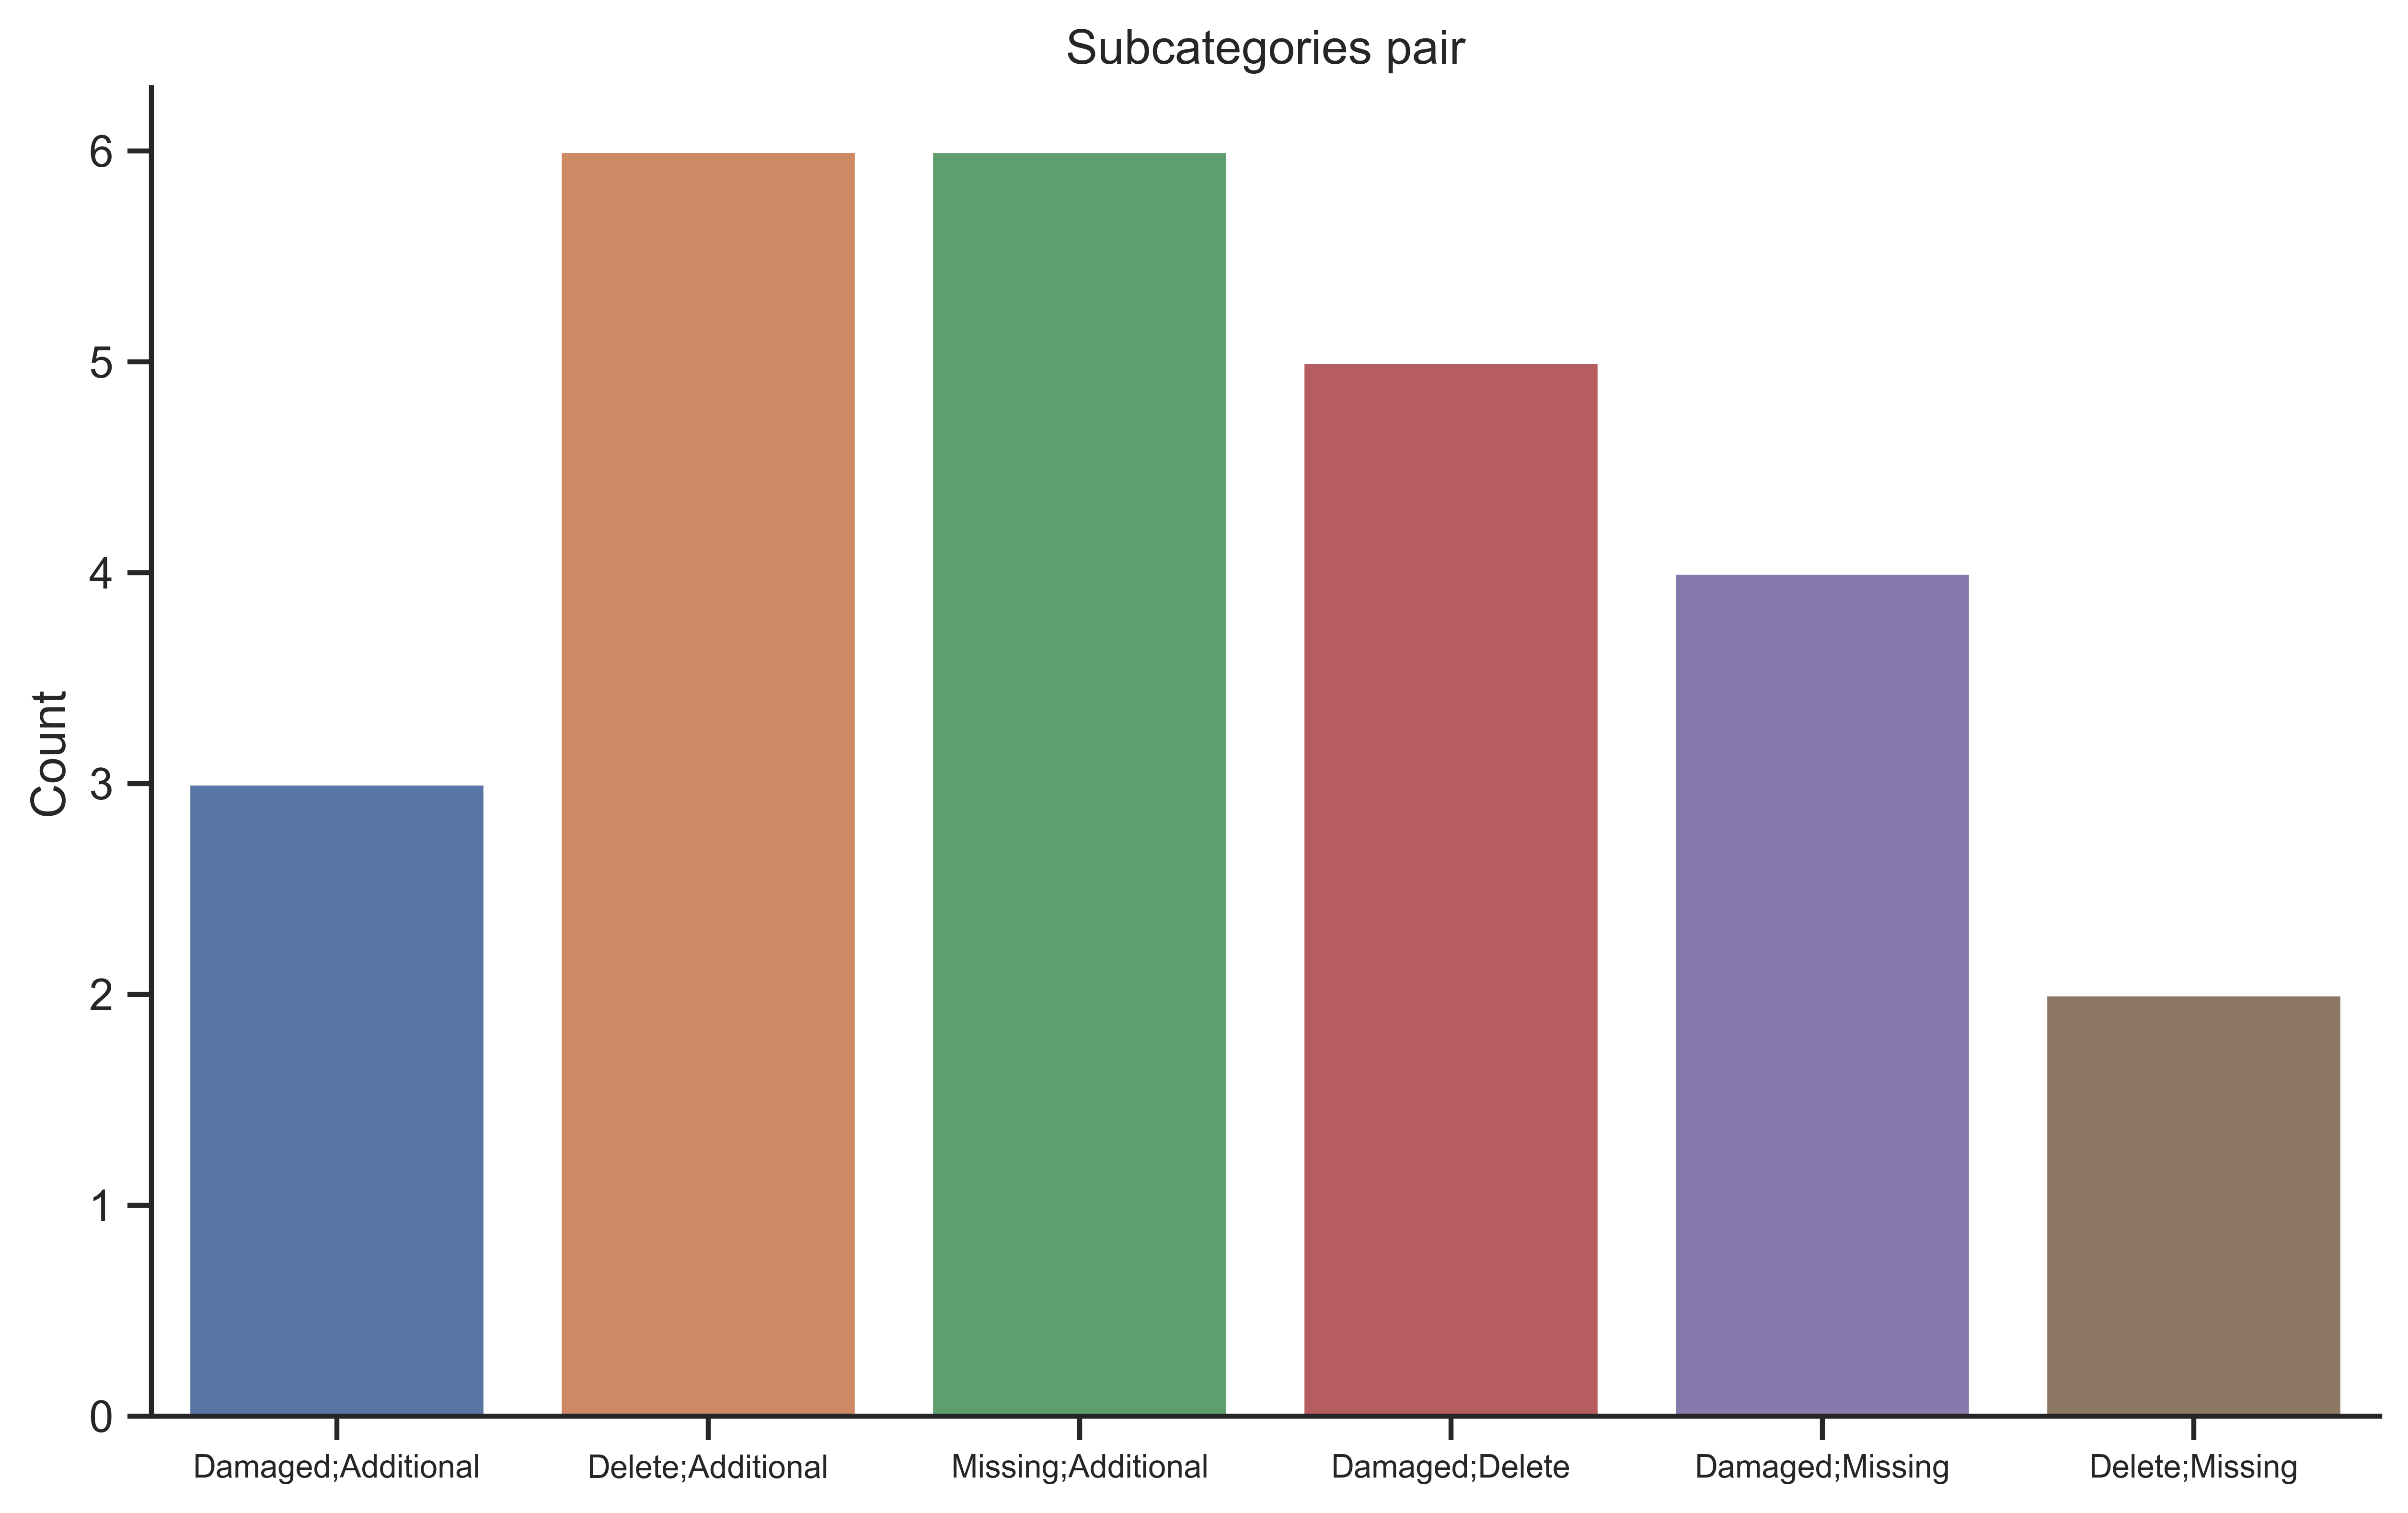
\includegraphics[width=\textwidth]{subcategory_pairs.png}
      \end{figure}
\end{center}
As we can see in most misclassification cases the "Garbage Collection: Additional Cart" is present. Specifically, the two most misclassified pairs are "Garbage Collection: Delete Cart" which is identified as "Garbage Collection: Additional Cart" and "Garbage Collection: Missing Cart" which is identified as "Garbage Collection: Additional Cart". The confusion is due to the strong similarity between subcategories: eg. an additional cart request could be due to a missing cart or a damaged cart, which means it's not necessarily easy to understand the correct category both for humans and GPT. We also hypothesized that sometimes there could be multiple correct categories.
\begin{center}
      \begin{figure}[ht]
            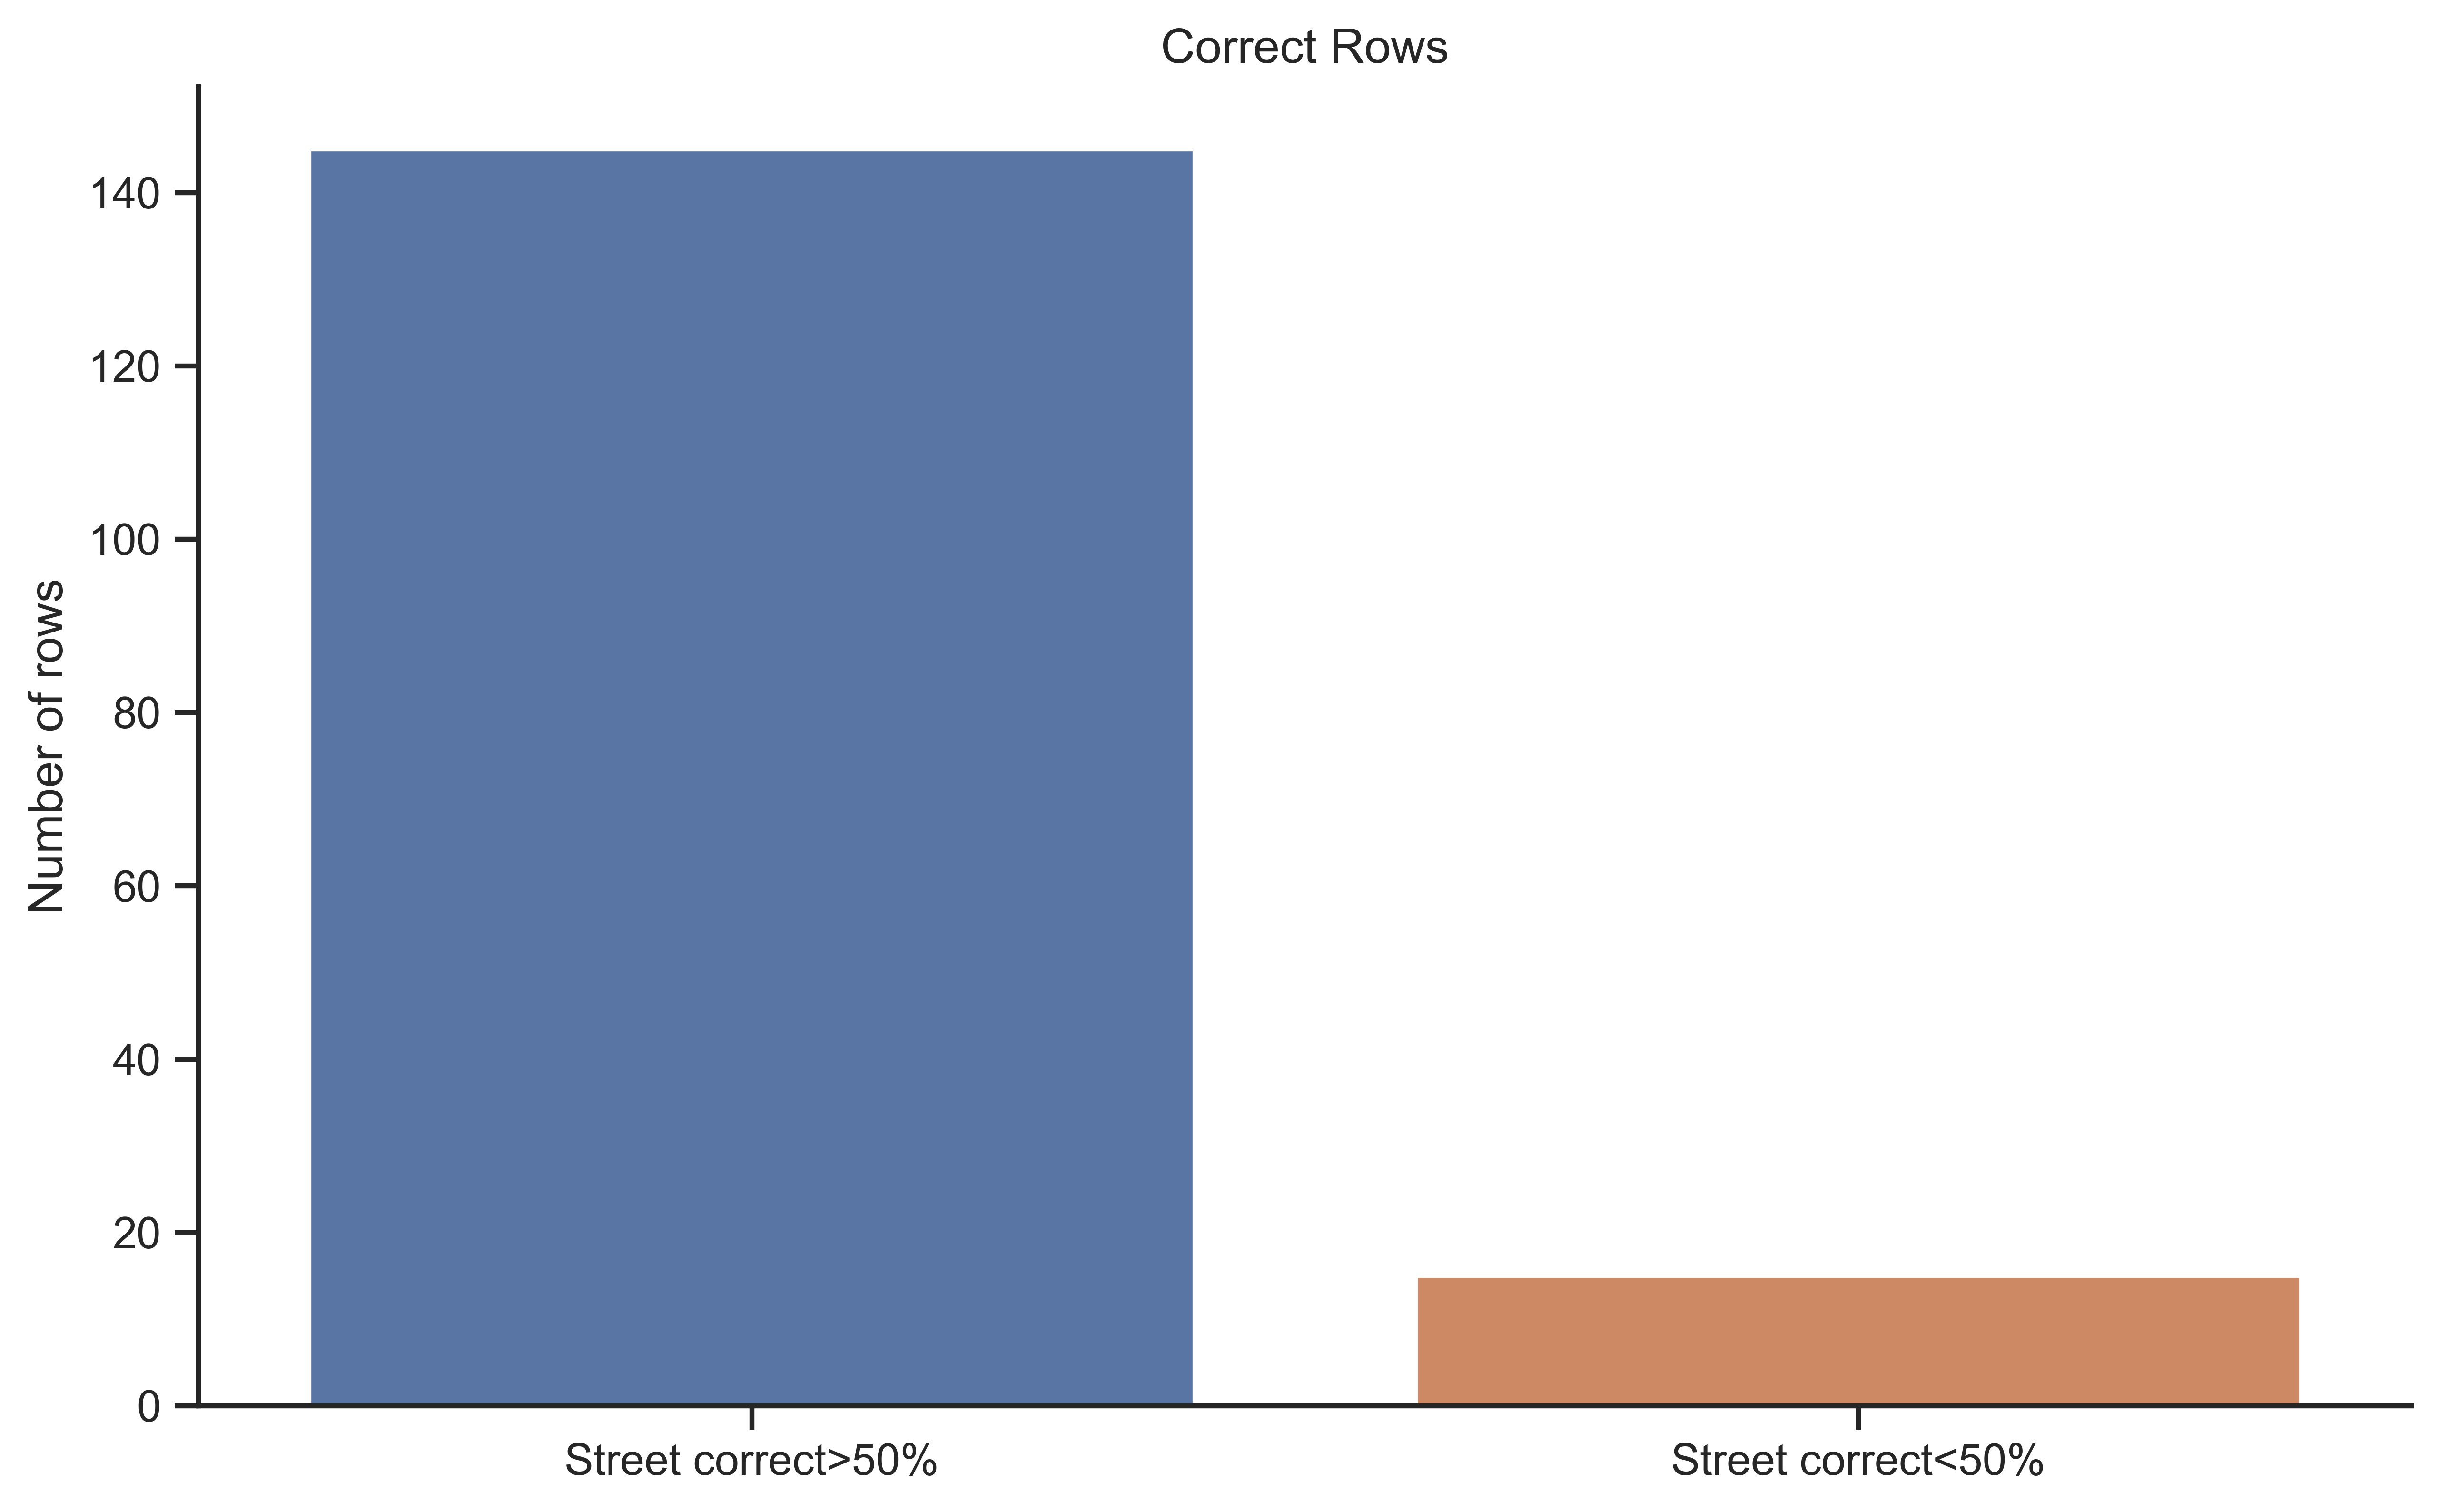
\includegraphics[width=0.99\textwidth]{street_recognition.png}
      \end{figure}
\end{center}
To evaluate the ability of the model to recognize the location in which the ticket request is taking place, we compared GPT's answer with a manually extracted label using the Python package fuzzywuzzy as specified in \ref{sec:techcomp}. This package gives a score from 0 to 100 based on how similar a certain string is with respect to the target string.
In most cases, GPT was able to find the correct street or set of streets, even if sometimes it wasn't able to infer the street type (Street, Avenue, Boulevard). In 90\% of cases, the correctness of the produced string was higher than 50/100. In most cases the string is classified with a score of 100, meaning the model is usually able to identify the street.
\begin{center}
      \begin{figure}[ht]
            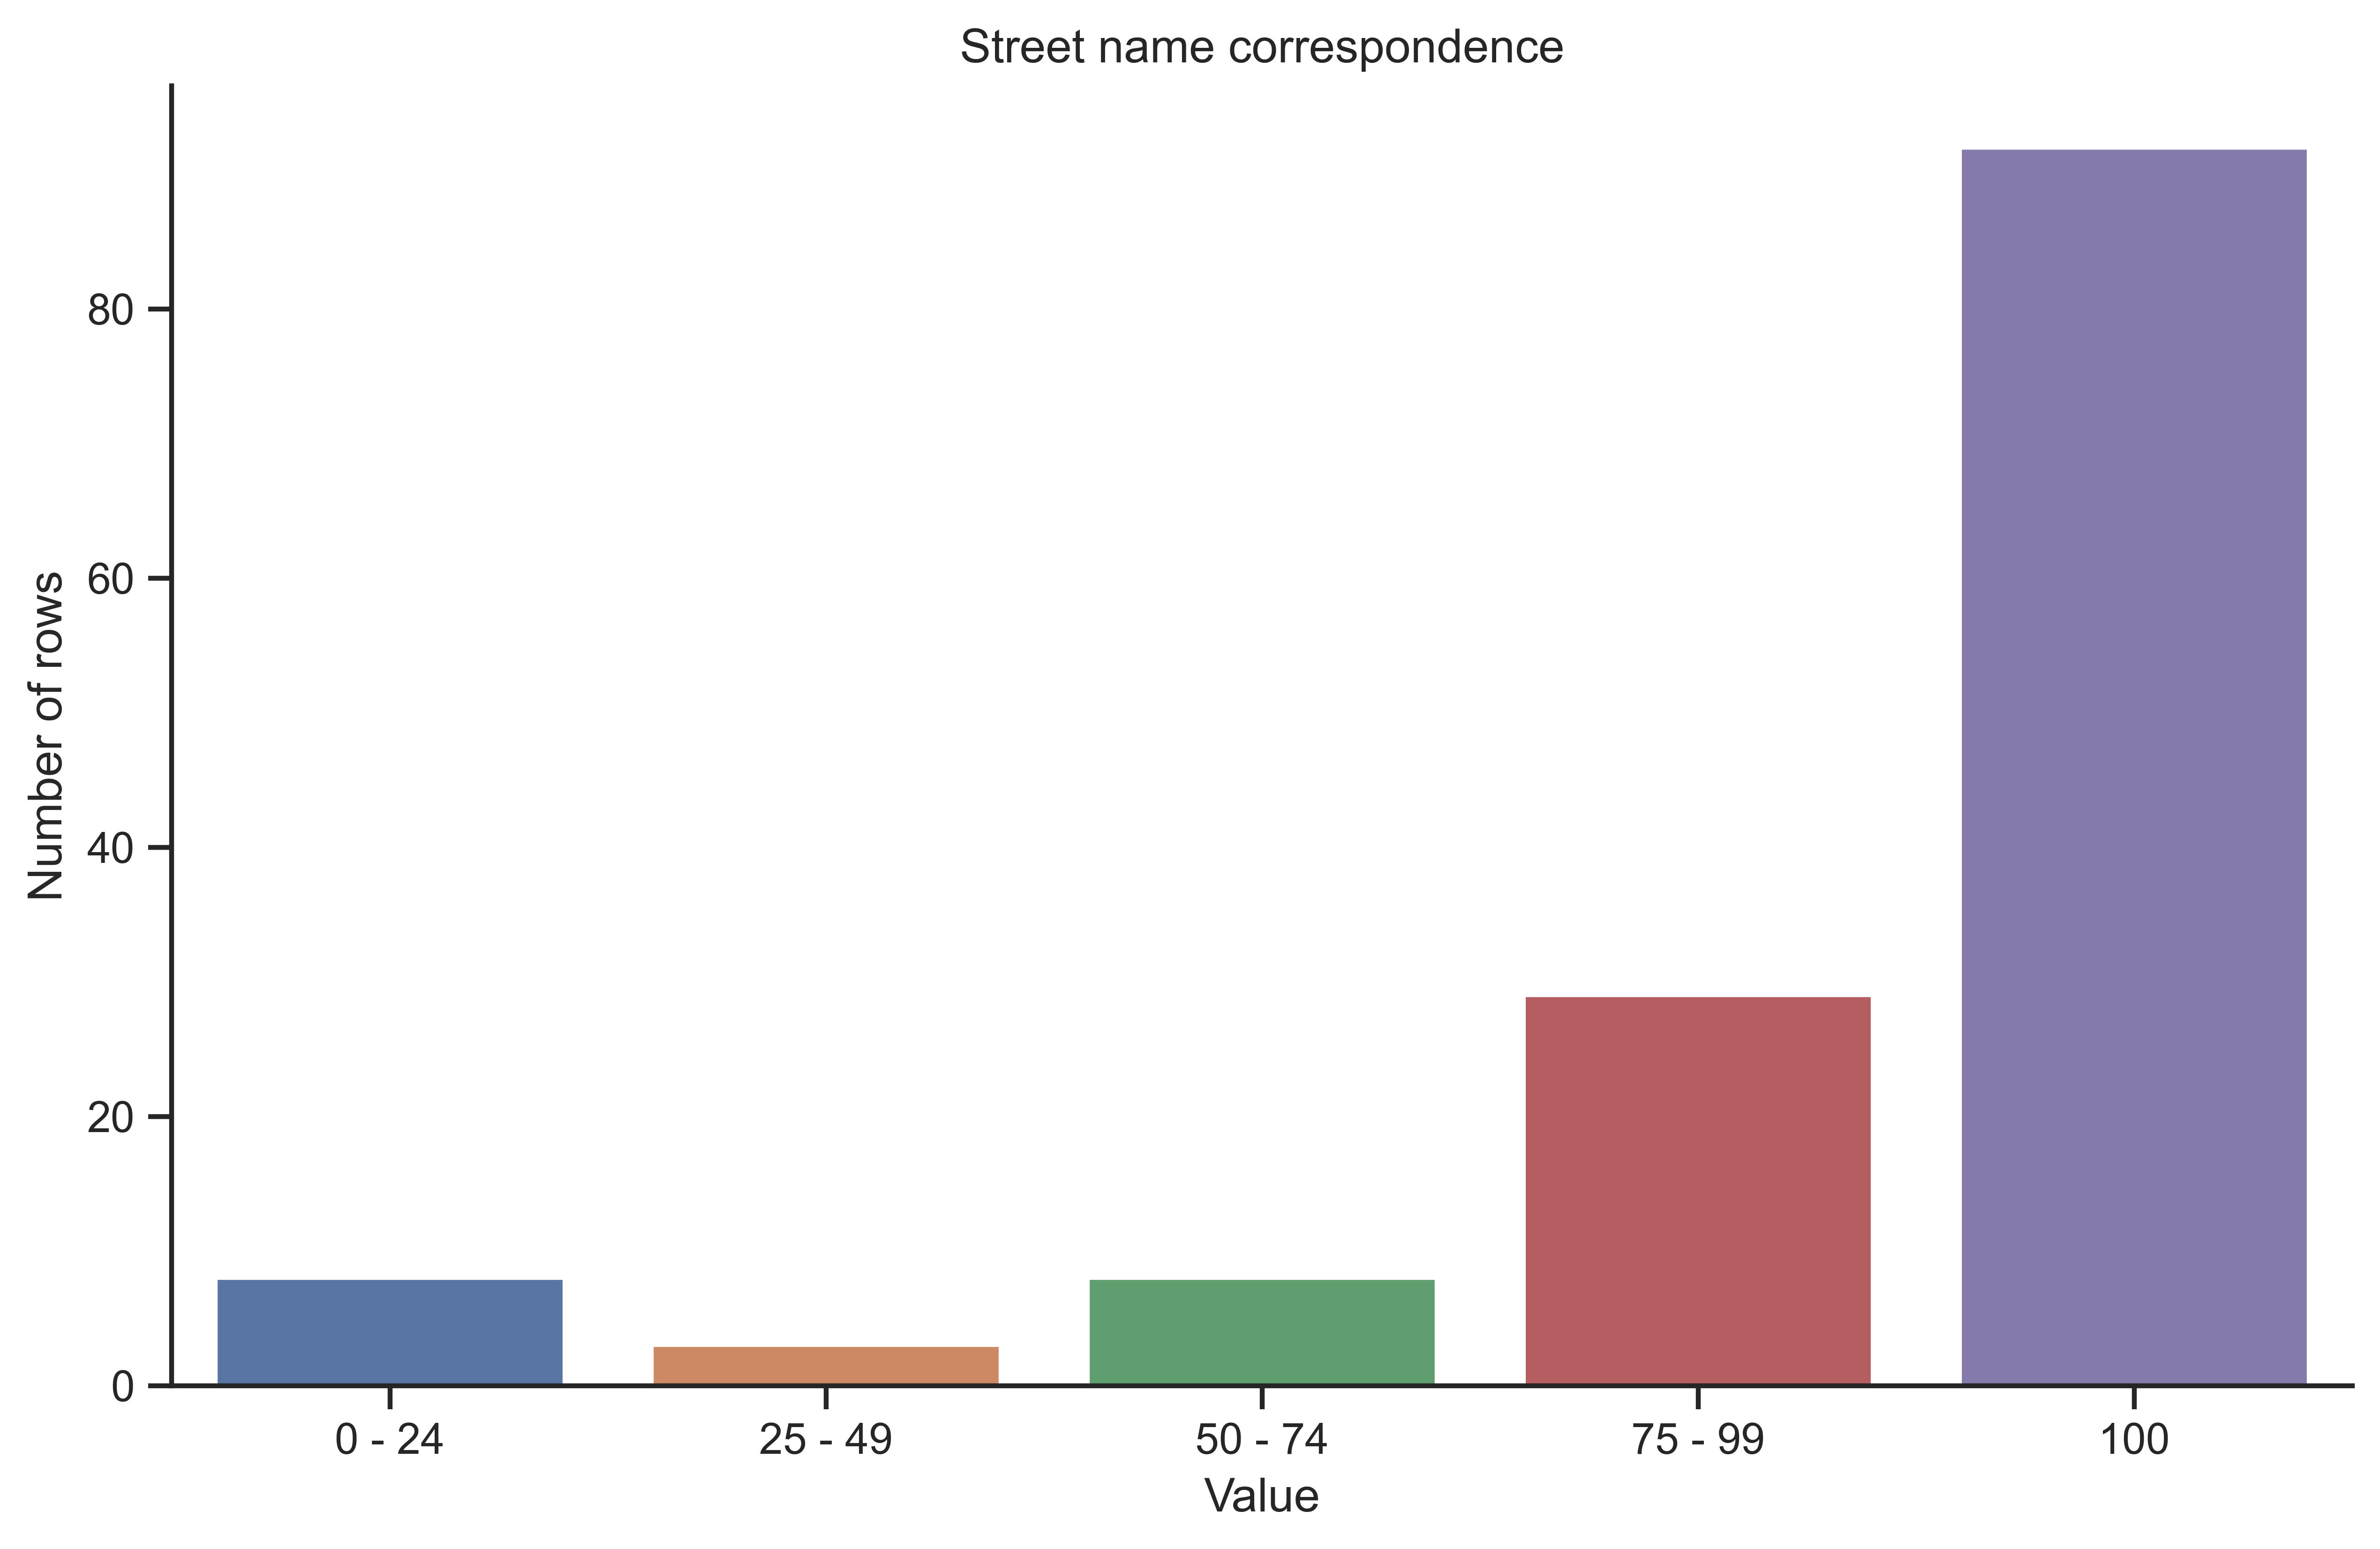
\includegraphics[width=0.99\textwidth]{street_correctness.png}
      \end{figure}
\end{center}

\newpage
\section{Problem Management Results}
\label{sec:probmanageres}
The prompt was structured as described before. The following are the questions:\\

\textit{Did the operator seem professional to you?                                                                                                          \\
      Is the number of days it took to resolve the problem greater than 2?                                                                                        \\
      Has the customer been updated on the ticket situation?                                                                                                      \\
      Has the technician found that the problem is attributable to the internal system (e.g. problems with the router or configurations) or to the external line? \\
      Was it necessary to involve the local technician externally?                                                                                                \\
      While resolving the issue, was it necessary to replace/change the router?                                                                                   \\
      Was the replaced router actually broken/faulty?}\\

The following are the obtained results:
\begin{center}
      \begin{tabular}{ccccccccccccccc}
            \toprule
            \# & Q1 & T\_Q1 & Q2 & T\_Q2 & Q3 & T\_Q3 & Q4 & T\_Q4 & Q5 & T\_Q5 & Q6 & T\_Q6 & Q7 & T\_Q7 \\
            \midrule
            1  & 1  & 1     & -1 & -1    & 1  & 1     & 0  & 0     & 2  & 2     & 0  & 0     & 0  & 0     \\
            2  & 1  & 1     & -1 & -1    & 1  & 1     & 1  & 1     & -2 & -2    & 0  & 0     & 0  & 0     \\
            3  & 1  & 1     & -1 & 1     & 1  & 1     & 1  & 1     & 2  & 2     & 1  & 1     & 1  & 1     \\
            4  & 1  & 1     & -1 & 1     & 1  & 1     & 1  & 1     & 2  & 2     & 0  & 0     & 0  & 0     \\
            5  & 1  & 1     & -1 & 1     & 1  & 1     & 0  & 0     & 2  & 2     & 0  & 0     & 0  & 0     \\
            6  & 1  & 1     & -1 & 1     & 1  & 1     & 0  & 0     & 2  & 2     & 0  & 0     & 0  & 0     \\
            7  & 1  & 1     & -1 & -1    & 1  & 1     & 1  & 1     & -2 & -2    & 1  & 1     & 1  & 1     \\
            8  & 1  & 1     & -1 & 1     & 1  & 1     & 1  & 1     & 2  & 2     & 0  & 0     & 0  & 0     \\
            9  & 1  & 1     & -1 & 1     & 1  & 1     & 0  & 0     & 2  & 2     & 0  & 0     & 0  & 0     \\
            10 & 1  & 1     & -1 & -1    & 1  & 1     & 1  & 1     & -2 & -2    & 1  & 1     & 1  & 1     \\
            \bottomrule
      \end{tabular}
\end{center}


\subsection{Problem management results comparison}

We choose RMSE to measure the error between GPT values and the expected ones, as this measure works well with regression problems. On the x-axis, we have the questions, while on the y-axis there are the RMSE values. The accuracy reached 90\%. As we can see, GPT always answers correctly to six out of seven questions; the only wrong one is the second question, which is about the overall ticket time resolution. This issue isn't hard to solve since the ticket-solving duration can be easily retrieved from the AEM Fiber system, as the domain expert suggested.

\chapter{List of Abbreviations}

\begin{description}
      \item[KIND:] Kindness
      \item[EXP:] Ability to explain themselves
      \item[SALE:] Initiative of the operator to make a pitch sale
      \item[SAT:] Customer satisfaction
      \item[TKIND:] Target Kindness
      \item[TEXP:] Target ability to explain themselves
      \item[TSALE:] Target initiative of the operator to make a pitch sale
      \item[TSAT:] Target customer satisfaction
      \item[OV:] Overall
      \item[TOV:] Target Overall
      \item[DIFF:] Difference between OV and TOV
      \item[CAT:] Category
      \item[TCAT:] Target Category
      \item[ICC:] Is Category Correct
      \item[STREET:] Street
      \item[TSTREET:] Target Street
      \item[STRSCORE:] Street Score
      \item[SUBC:] Subcategory
      \item[TSUBC:] Target Subcategory
      \item[ISC:] Is Subcategory Correct
      \item[Q\#:] Answer to question number \#
      \item[T\_Q\#:] Target answer to question number \#
\end{description}
\bibliographystyle{plain} % We choose the "plain" reference style
\bibliography{refs} % Entries are in the refs.bib file
\end{document}